%Version 3 October 2023
% See section 11 of the User Manual for version history
%
%%%%%%%%%%%%%%%%%%%%%%%%%%%%%%%%%%%%%%%%%%%%%%%%%%%%%%%%%%%%%%%%%%%%%%
%%                                                                 %%
%% Please do not use \input{...} to include other tex files.       %%
%% Submit your LaTeX manuscript as one .tex document.              %%
%%                                                                 %%
%% All additional figures and files should be attached             %%
%% separately and not embedded in the \TeX\ document itself.       %%
%%                                                                 %%
%%%%%%%%%%%%%%%%%%%%%%%%%%%%%%%%%%%%%%%%%%%%%%%%%%%%%%%%%%%%%%%%%%%%%

%%\documentclass[referee,sn-basic]{sn-jnl}% referee option is meant for double line spacing

%%=======================================================%%
%% to print line numbers in the margin use lineno option %%
%%=======================================================%%

%%\documentclass[lineno,sn-basic]{sn-jnl}% Basic Springer Nature Reference Style/Chemistry Reference Style

%%======================================================%%
%% to compile with pdflatex/xelatex use pdflatex option %%
%%======================================================%%

%%\documentclass[pdflatex,sn-basic]{sn-jnl}% Basic Springer Nature Reference Style/Chemistry Reference Style


%%Note: the following reference styles support Namedate and Numbered referencing. By default the style follows the most common style. To switch between the options you can add or remove �Numbered� in the optional parenthesis. 
%%The option is available for: sn-basic.bst, sn-vancouver.bst, sn-chicago.bst%  
 
%%\documentclass[sn-nature]{sn-jnl}% Style for submissions to Nature Portfolio journals
%%\documentclass[sn-basic]{sn-jnl}% Basic Springer Nature Reference Style/Chemistry Reference Style
%%\documentclass[sn-mathphys-num]{sn-jnl}% Math and Physical Sciences Numbered Reference Style 
%%\documentclass[sn-mathphys-ay]{sn-jnl}% Math and Physical Sciences Author Year Reference Style
%%\documentclass[sn-aps]{sn-jnl}% American Physical Society (APS) Reference Style
%%\documentclass[sn-vancouver,Numbered]{sn-jnl}% Vancouver Reference Style
\documentclass[pdflatex,sn-apa]{sn-jnl}% APA Reference Style 
%%\documentclass[sn-chicago]{sn-jnl}% Chicago-based Humanities Reference Style

%%%% Standard Packages
%%<additional latex packages if required can be included here>

\usepackage{graphicx}%
\usepackage{multirow}%
\usepackage{amsmath,amssymb,amsfonts}%
%% \usepackage{amsmath,amssymb,amsfonts}%
\usepackage{amsthm}%
\usepackage{mathrsfs}%
\usepackage[title]{appendix}%
\usepackage{xcolor}%
\usepackage{textcomp}%
\usepackage{manyfoot}%
\usepackage{booktabs}%
%% \usepackage{algorithm}%
%% \usepackage{algorithmicx}%
%% \usepackage{algpseudocode}%
\usepackage{listings}%
\usepackage{placeins}
%%%%
\newtheorem*{definition}{Definition}
\DeclareMathOperator*{\argmax}{argmax}
\DeclareMathOperator*{\argmin}{argmin}
\DeclareMathOperator{\sgn}{sgn}


%%%%%=============================================================================%%%%
%%%%  Remarks: This template is provided to aid authors with the preparation
%%%%  of original research articles intended for submission to journals published 
%%%%  by Springer Nature. The guidance has been prepared in partnership with 
%%%%  production teams to conform to Springer Nature technical requirements. 
%%%%  Editorial and presentation requirements differ among journal portfolios and 
%%%%  research disciplines. You may find sections in this template are irrelevant 
%%%%  to your work and are empowered to omit any such section if allowed by the 
%%%%  journal you intend to submit to. The submission guidelines and policies 
%%%%  of the journal take precedence. A detailed User Manual is available in the 
%%%%  template package for technical guidance.
%%%%%=============================================================================%%%%

%% as per the requirement new theorem styles can be included as shown below
%%\theoremstyle{thmstyleone}%
%%\newtheorem{theorem}{Theorem}%  meant for continuous numbers
%%\newtheorem{theorem}{Theorem}[section]% meant for sectionwise numbers
%% optional argument [theorem] produces theorem numbering sequence instead of independent numbers for Proposition
%%\newtheorem{proposition}[theorem]{Proposition}% 
%%\newtheorem{proposition}{Proposition}% to get separate numbers for theorem and proposition etc.

%%\theoremstyle{thmstyletwo}%
%%\newtheorem{example}{Example}%
%%\newtheorem{remark}{Remark}%

%%\theoremstyle{thmstylethree}%
%%\newtheorem{definition}{Definition}%

\raggedbottom
%%\unnumbered% uncomment this for unnumbered level heads

\begin{document}

\title[Location and Scale-Invariant Power Transformations for Transforming Data to Normality]{Location and Scale-Invariant Power Transformations for Transforming Data to Normality}

%%=============================================================%%
%% GivenName	-> \fnm{Joergen W.}
%% Particle	-> \spfx{van der} -> surname prefix
%% FamilyName	-> \sur{Ploeg}
%% Suffix	-> \sfx{IV}
%% \author*[1,2]{\fnm{Joergen W.} \spfx{van der} \sur{Ploeg} 
%%  \sfx{IV}}\email{iauthor@gmail.com}
%%=============================================================%%

\author*[1,2]{\fnm{Alex} \sur{Zwanenburg}}\email{alexander.zwanenburg@nct-dresden.de}

\author[2,3,4]{\fnm{Steffen} \sur{L{\"o}ck}}\email{steffen.loeck@oncoray.de}

\affil*[1]{
	\orgdiv{National Center for Tumor Diseases (NCT), NCT/UCC Dresden },
	\orgname{a partnership between DKFZ, Faculty of
	Medicine and University Hospital Carl Gustav Carus, TUD Dresden University of Technology, and
	Helmholtz-Zentrum Dresden-Rossendorf (HZDR)},
	\orgaddress{\street{Fetscherstra{\ss}e 74/PF 64}, \city{Dresden}, \postcode{01307}, \country{Germany}}
}

\affil[2]{
	\orgdiv{OncoRay - National Center for Radiation Research in Oncology}
	\orgname{Faculty of Medicine and University Hospital Carl Gustav Carus, TUD Dresden University of Technology,
    Helmholtz-Zentrum Dresden-Rossendorf},
	\orgaddress{\street{Fetscherstra{\ss}e 74/PF 41}, \city{Dresden}, \postcode{01307}, \country{Germany}}
}

\affil[3]{
	\orgdiv{Department of Radiotherapy and Radiation Oncology},
	\orgname{Faculty of Medicine and University Hospital Carl Gustav Carus, TUD Dresden University of Technology},
	\orgaddress{\street{Fetscherstra{\ss}e 74/PF 50}, \city{Dresden}, \postcode{01307}, \country{Germany}}
}

\affil[4]{
	\orgdiv{German Cancer Consortium (DKTK), Partner Site Dresden},
	\orgname{German Cancer Research Center (DKFZ)},
	\orgaddress{\street{Im Neuenheimer Feld 280}, \city{Heidelberg}, \postcode{69192}, \country{Germany}}
}

%%==================================%%
%% Sample for unstructured abstract %%
%%==================================%%

\abstract{Power transformations are used to stabilize variance and achieve
normality of features, especially in methods assuming normal
distributions such as ANOVA and linear discriminant analysis. However,
the commonly used Box-Cox and Yeo-Johnson power transformation methods
are sensitive to the location, scale, and presence of outliers in the
data. Here we present location- and scale-invariant Box-Cox and
Yeo-Johnson transformations to mitigate these issues. We derive maximum
likelihood estimation criteria for optimizing transformation parameters
and propose robust adaptations that reduce the influence of outliers. We
also introduce an empirical test for assessing central normality of
transformed features. In simulations and real-world datasets, robust
location- and scale-invariant transformations outperform conventional
variants, resulting in better transformations to central normality. In a
machine learning experiment with 231 datasets with numerical features,
integrating robust location- and scale-invariant power transformations
into an automated data processing and machine learning pipeline did not
result in a meaningful improvement or detriment to model performance
compared to conventional variants. In conclusion, robust location- and
scale-invariant power transformations can replace conventional variants.}

%%================================%%
%% Sample for structured abstract %%
%%================================%%

% \abstract{\textbf{Purpose:} The abstract serves both as a general introduction to the topic and as a brief, non-technical summary of the main results and their implications. The abstract must not include subheadings (unless expressly permitted in the journal's Instructions to Authors), equations or citations. As a guide the abstract should not exceed 200 words. Most journals do not set a hard limit however authors are advised to check the author instructions for the journal they are submitting to.
% 
% \textbf{Methods:} The abstract serves both as a general introduction to the topic and as a brief, non-technical summary of the main results and their implications. The abstract must not include subheadings (unless expressly permitted in the journal's Instructions to Authors), equations or citations. As a guide the abstract should not exceed 200 words. Most journals do not set a hard limit however authors are advised to check the author instructions for the journal they are submitting to.
% 
% \textbf{Results:} The abstract serves both as a general introduction to the topic and as a brief, non-technical summary of the main results and their implications. The abstract must not include subheadings (unless expressly permitted in the journal's Instructions to Authors), equations or citations. As a guide the abstract should not exceed 200 words. Most journals do not set a hard limit however authors are advised to check the author instructions for the journal they are submitting to.
% 
% \textbf{Conclusion:} The abstract serves both as a general introduction to the topic and as a brief, non-technical summary of the main results and their implications. The abstract must not include subheadings (unless expressly permitted in the journal's Instructions to Authors), equations or citations. As a guide the abstract should not exceed 200 words. Most journals do not set a hard limit however authors are advised to check the author instructions for the journal they are submitting to.}

\keywords{Data preprocessing, Feature transformation, Outliers, Power transformation}

%%\pacs[JEL Classification]{D8, H51}

%%\pacs[MSC Classification]{35A01, 65L10, 65L12, 65L20, 65L70}

\maketitle

\section{Introduction}\label{introduction}

Many statistical and some machine learning methods assume normality of
the underlying data, e.g.~analysis of variance and linear discriminant
analysis. However, numerical features in datasets may strongly deviate
from normal distributions, e.g.~by being skewed. Power transformations
aim to stabilise variance and improve normality of such features
\citep{Bartlett1947-rx, Tukey1957-rt}. The two most commonly used
transformations are that of \citet{Box1964-mz} and \citet{Yeo2000-vw}.

The Box-Cox transformation is defined as:

\begin{definition}[Box-Cox power transformation]
Let $\mathbf{X} = \left\{x_1, x_2, \ldots, x_n | x_i > 0 \right\}$ be a finite sequence of length $n > 0$.
Let $\lambda \in \mathcal{R}$ be a transformation parameter.
Then the Box-Cox power transformation of element $x_i$ is defined as:
\begin{equation}
\label{eqn:box-cox-original}
\phi_{\text{BC}}^\lambda (x_i) = 
\begin{cases}
\left(x_i^\lambda - 1 \right) / \lambda & \text{if } \lambda \neq 0\\
\log(x_i) & \text{if } \lambda = 0
\end{cases}
\end{equation}
\end{definition}

One limitation of the Box-Cox transformation is that it is only defined
for \(x_i > 0\). In contrast, the Yeo-Johnson transformation under the
transformation parameter \(\lambda\) is defined for any
\(x_i \in \mathbb{R}\), as follows:

\begin{definition}[Yeo-Johnson power transformation]
Let $\mathbf{X} = \left\{x_1, x_2, \ldots, x_n | x_i \in \mathbb{R} \right\}$ be a finite sequence of length $n > 0$.
Let $\lambda \in \mathcal{R}$ be a transformation parameter.
\begin{equation}
\label{eqn:yeo-johnson-original}
\phi_{\text{YJ}}^\lambda (x_i) = 
\begin{cases}
\left( \left( 1 + x_i \right)^\lambda - 1\right) / \lambda & \text{if } \lambda \neq 0 \text{ and } x_i \geq 0\\
\log(1 + x_i) & \text{if } \lambda = 0 \text{ and } x_i \geq 0\\
-\left( \left( 1 - x_i\right)^{2 - \lambda} - 1 \right) / \left(2 - \lambda \right) & \text{if } \lambda \neq 2 \text{ and } x_i < 0\\
-\log(1 - x_i) & \text{if } \lambda = 2 \text{ and } x_i < 0
\end{cases}
\end{equation}
\end{definition}

The \(\lambda\)-parameter is typically optimised using maximum
likelihood estimation under the assumption that the transformed feature
is normally distributed. As noted by Raymaekers and Rousseeuw, this
approach is sensitive to outliers, and robust versions of Box-Cox and
Yeo-Johnson transformations were devised \citep{Raymaekers2024-zf}.

Applying a power transformation does not guarantee that transformed
features are normally distributed. Depending on location and scale of a
feature and the presence of outliers, power transformations may decrease
normality, as shown in Figure \ref{fig:decreased-normality}. If
normality of the transformed feature is not checked, e.g.~in automated
power transformation in machine learning workflows, several issues may
arise. For example, statistical tests such as ANOVA may produce
incorrect results due to violation of the normality assumption.
Likewise, machine learning methods that assume normality of input
features may suffer a decrease in performance. Moreover, large negative
or positive \(\lambda\)-parameters may lead to numeric issues in any
subsequent computations.

Statistical tests for normality, such as the Shapiro-Wilk test \citep{Shapiro1965-zd},
could be automatically applied to transformed features.
However, given sufficiently large sample sizes such tests can detect
trivial deviations from normality, and may lead to rejection of
sufficiently good power transformations.

\begin{figure}

{\centering 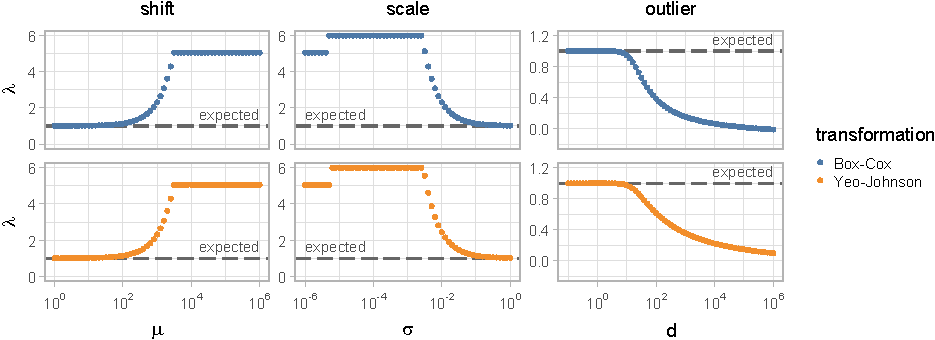
\includegraphics[width=1\linewidth]{figure_1} 

}

\caption{Effect of location, scale and outliers on estimation of the Box-Cox and Yeo-Johnson transformation parameter $\lambda$. $10000$ samples were drawn from a normal distribution: $\mathcal{N}(\mu, 1)$ for the \textit{shift} dataset, $\mathcal{N}(10, \sigma)$ for the \textit{scale} dataset and $\mathcal{N}(0, 1)$ for the \textit{outlier} dataset. Additionally, an outlier with value $d$ was added to the outlier dataset. Since samples are drawn from a normal distribution, a transformation parameter of $\lambda = 1$ is expected. However, a large shift in location, a scale that is small compared to the location, or presence of large outliers lead to incorrectly estimated transformation parameter values.}\label{fig:decreased-normality}
\end{figure}

To address these issues, we make the following contributions:

\begin{itemize}
\item
  We devise location- and scale-invariant versions of the Box-Cox and
  Yeo-Johnson transformation, including versions robust to outliers.
\item
  We derive the maximum likelihood criterion for location- and
  scale-invariant Box-Cox and Yeo-Johnson transformations to allow for
  optimising transformation parameters.
\item
  We define an empirical central normality test for detecting cases
  where power transformations fail to yield an approximately normally
  distributed transformed feature.
\item
  We assess the effect of power transformations on the performance of
  machine learning models.
\end{itemize}

\section{Theory}\label{theory}

In this section, we will first introduce location- and scale-invariant
versions of the Box-Cox and Yeo-Johnson transformations. Subsequently,
we define weighted location- and scale-invariant transformations and
weighting methods for robust transformations. We then define the
quantile function for asymmetric generalised normal distributions to
enable random sampling. Finally, we define the overall framework for the
empirical central normality test.

First, we define a (numeric) feature. Throughout this work, whenever
reference is made to a feature, a numeric feature is meant unless noted
otherwise.

\begin{definition}[Numeric feature]
A numeric feature is a finite sequence $\mathbf{X} = \left\{x_1, x_2, \ldots, x_n | x_i \in  \right\}$ of length $n$.
\end{definition}

\subsection{Location- and scale-invariant power
transformation}\label{location--and-scale-invariant-power-transformation}

Box-Cox and Yeo-Johnson transformations are modified by introducing
shift parameter \(x_0\) and scale parameter \(s\) into equations
\ref{eqn:box-cox-original} and \ref{eqn:yeo-johnson-original}. The
location- and scale-invariant Box-Cox transformation of a feature value
\(x_i\) of feature \(\mathbf{X}\) under transformation parameter
\(\lambda\), shift parameter \(x_0\) and scale parameter \(s\) is then
defined as:

\begin{definition}[Location- and scale- invariant Box-Cox power transformation]
Let $\lambda \in \mathcal{R}$ be a transformation parameter.
Let $x_0 \in \mathcal{R}$ and $s > 0$ be location and scale parameters.
Let $\mathbf{X} = \left\{x_1, x_2, \ldots, x_n | x_i - x_0 > 0 \right\}$ be a finite sequence of length $n > 0$.

Then the location- and scale-invariant Box-Cox power transformation of element $x_i$ is defined as:

\begin{equation}
\label{eqn:box-cox-invariant}
\phi_{\text{BC}}^{\lambda, x_0, s} (x_i) = 
\begin{cases}
\left( \left(\frac{x_i - x_0}{s} \right)^\lambda - 1 \right) / \lambda & \text{if } \lambda \neq 0\\
\log\left[\frac{x_i - x_0}{s}\right] & \text{if } \lambda = 0
\end{cases}
\end{equation}
\end{definition}

Likewise, the location- and scale-invariant Yeo-Johnson transformation
of a feature value \(x_i\) under transformation parameter \(\lambda\),
shift parameter \(x_0\) and scale parameter \(s\) is defined as:

\begin{definition}[Location- and scale- invariant Yeo-Johnson power transformation]
Let $\lambda \in \mathcal{R}$ be a transformation parameter.
Let $x_0 \in \mathcal{R}$ and $s > 0$ be location and scale parameters.
Let $\mathbf{X} = \left\{x_1, x_2, \ldots, x_n | x_i \in \mathcal{R} \right\}$ be a finite sequence of length $n > 0$.

Then the location- and scale-invariant Yeo-Johnson power transformation of element $x_i$ is defined as:

\begin{equation}
\label{eqn:yeo-johnson-invariant}
\phi_{\text{YJ}}^{\lambda, x_0, s} (x_i) = 
\begin{cases}
\left( \left( 1 + \frac{x_i - x_0}{s}\right)^\lambda - 1\right) / \lambda & \text{if } \lambda \neq 0 \text{ and } x_i - x_0 \geq 0\\
\log\left[1 + \frac{x_i - x_0}{s}\right] & \text{if } \lambda = 0 \text{ and } x_i - x_0 \geq 0\\
-\left( \left( 1 - \frac{x_i - x_0}{s}\right)^{2 - \lambda} - 1 \right) / \left(2 - \lambda \right) & \text{if } \lambda \neq 2 \text{ and } x_i - x_0 < 0\\
-\log\left[1 - \frac{x_i - x_0}{s}\right] & \text{if } \lambda = 2 \text{ and } x_i - x_0 < 0
\end{cases}
\end{equation}
\end{definition}

For both invariant transformations, \(\lambda\), \(x_0\) and \(s\)
parameters can be obtained by maximising the log-likelihood function,
i.e.~using maximum likelihood estimation (MLE). A full derivation of the
log-likelihood function for both transformations is shown in \hyperref[appendix-a]{Appendix A}.
The location- and scale-invariant Box-Cox log-likelihood function is:

\begin{definition} [Log-likelihood function of the location- and scale- invariant Box-Cox power transformation]
Let $\mathbf{X}$, $\lambda$, $x_0$, and $s$ be defined as earlier (Eqn. \ref{eqn:box-cox-invariant}).
Let $\mu$ and $\sigma^2$ be the mean and variance of the transformed sequence $\phi_{\text{BC}}^{\lambda, x_0, s} (\mathbf{X})$, respectively.

Then the log-likelihood function of the location- and scale- invariant Box-Cox power transformation is defined as:
\begin{equation}
\label{eqn:box-cox-invariant-log-likelihood}
\begin{split}
\mathcal{L}_{\text{BC}}^{\lambda, x_0, s} = & -\frac{n}{2} \log \left[2 \pi \sigma^2 \right] -\frac{1}{2 \sigma^2} \sum_{i=1}^n \left( \phi_{BC}^{\lambda, x_0, s}(x_i) - \mu \right)^2 \\
& -n \lambda \log s + \left( \lambda - 1 \right) \sum_{i=1}^n \log \left[ x_i - x_0 \right]
\end{split}
\end{equation}
\end{definition}

Similarly, the location- and scale-invariant Yeo-Johnson log-likelihood
function is:

\begin{definition}[Log-likelihood function of the location- and scale- invariant Yeo-Johnson power transformation]
Let $\mathbf{X}$, $\lambda$, $x_0$, and $s$ be defined as earlier (Eqn. \ref{eqn:yeo-johnson-invariant}).
Let $\mu$ and $\sigma^2$ be the mean and variance of the transformed sequence $\phi_{\text{YJ}}^{\lambda, x_0, s} (\mathbf{X})$, respectively.

Then the log-likelihood function of the location- and scale- invariant Yeo-Johnson power transformation is defined as:
\begin{equation}
\label{eqn:yeo-johnson-invariant-log-likelihood}
\begin{split}
\mathcal{L}_{\text{YJ}}^{\lambda, x_0, s} = & -\frac{n}{2} \log\left[2 \pi \sigma^2\right] -\frac{1}{2 \sigma^2} \sum_{i=1}^n \left( \phi_{YJ}^{\lambda, x_0, s}(x_i) - \mu \right)^2 \\
& - n \log s + (\lambda - 1) \sum_{i=1}^n \mathop{\mathrm{sgn}}(x_i - x_0) \log \left[1 + \frac{|x_i - x_0|}{s} \right]
\end{split}
\end{equation}
\end{definition}




\subsection{Robust location- and scale-invariant power
transformations}\label{robust-location--and-scale-invariant-power-transformations}

Real-world data may contain outliers, to which maximum likelihood
estimation can be sensitive. Their presence may lead to poor
transformations to normality, as shown in Figure
\ref{fig:decreased-normality}. As indicated by \citet{Raymaekers2024-zf},
 the general aim of power transformations should be to transform
non-outlier data to normality, i.e.~achieve \emph{central normality}. To
achieve this, they devised an iterative procedure to find a robust
estimate of the transformation parameter \(\lambda\). Briefly, this
process requires identifying outliers in the data and weighting such
instances during the optimisation process. \citet{Raymaekers2024-zf}
achieve this through weighted maximum likelihood estimation.
However, because this procedure iteratively estimates and updates
\(\lambda\), it can not be used here to simultaneously estimate
\(\lambda\), \(x_0\) and \(s\) for location- and scale-invariant power
transformations. Nonetheless, as a procedure, weighted MLE can be used
for estimating the transformation, shift and scale parameters.

Here, weighted maximum likelihood estimation is based on equations
\ref{eqn:box-cox-invariant-log-likelihood} and
\ref{eqn:yeo-johnson-invariant-log-likelihood}. Compared to \citet{Raymaekers2024-zf},
these log-likelihood functions include additional
terms to accommodate estimation of \(x_0\) and \(s\). The weighted
location- and scale-invariant Box-Cox log-likelihood function is:

\begin{definition}[Weighted log-likelihood function of the location- and scale- invariant Box-Cox power transformation]
Let $\mathbf{X}$, $\lambda$, $x_0$, and $s$ be defined as earlier (Eqn. \ref{eqn:box-cox-invariant}).
Let $w_i \geq 0$ be the weight corresponding to each element of $\mathbf{X}$.
Let $\mu_w$ be the weighted mean of the Box-Cox transformed sequence:
\begin{equation*}
\mu_w = \frac{\sum_{i=1}^n w_i \phi_{\text{BC}}^{\lambda, x_0, s} (x_i)} {\sum_{i=1}^n w_i}
\end{equation*}

Let $\sigma^2_w$ be the weighted variance of the Box-Cox transformed sequence:
\begin{equation*}
\sigma_w^2 = \frac{\sum_{i=1}^n w_i \left(\phi_{\text{BC}}^{\lambda, x_0, s} (x_i) - \mu_w \right)^2}{\sum_{i=1}^n w_i}
\end{equation*}

Then, the weighted log-likelihood function of the location- and scale- invariant Box-Cox power transformation is:

\begin{equation}
\label{eqn:box-cox-weighted-invariant-log-likelihood}
\begin{split}
\mathcal{L}_{\text{rBC}}^{\lambda, x_0, s} = & -\frac{1}{2} \left(\sum_{i=1}^n w_i \right) \log \left[ 2 \pi \sigma_w^2 \right] -\frac{1}{2 \sigma_w^2} \sum_{i=1}^n w_i \left( \phi_{\text{BC}}^{\lambda, x_0, s}(x_i) - \mu_w \right)^2 \\
& - \lambda \left( \sum_{i=1}^n w_i \right) \log s + \left( \lambda - 1 \right) \sum_{i=1}^n w_i \log \left[ x_i - x_0 \right]
\end{split}
\end{equation}
\end{definition}

Analogously, the weighted location- and scale-invariant Yeo-Johnson
log-likelihood function is:

\begin{definition}[Weighted log-likelihood function of the location- and scale- invariant Yeo-Johnson power transformation]

Let $\mathbf{X}$, $\lambda$, $x_0$, and $s$ be defined as earlier (Eqn. \ref{eqn:yeo-johnson-invariant}).
Let $w_i \geq 0$ be the weight corresponding to each element of $\mathbf{X}$.
Let $\mu_w$ be the weighted mean of the Yeo-Johnson transformed sequence:
\begin{equation*}
\mu_w = \frac{\sum_{i=1}^n w_i \phi_{\text{YJ}}^{\lambda, x_0, s} (x_i)} {\sum_{i=1}^n w_i}
\end{equation*}

Let $\sigma^2_w$ be the weighted variance of the Yeo-Johnson transformed sequence:
\begin{equation*}
\sigma_w^2 = \frac{\sum_{i=1}^n w_i \left(\phi_{\text{YJ}}^{\lambda, x_0, s} (x_i) - \mu_w \right)^2}{\sum_{i=1}^n w_i}
\end{equation*}

Then, the weighted log-likelihood function of the location- and scale- invariant Yeo-Johnson power transformation is:

\begin{equation}
\label{eqn:yeo-johnson-weighted-invariant-log-likelihood}
\begin{split}
\mathcal{L}_{\text{rYJ}}^{\lambda, x_0, s} = & -\frac{1}{2} \left(\sum_{i=1}^n w_i \right) \log \left[ 2 \pi \sigma_w^2 \right] -\frac{1}{2 \sigma_w^2} \sum_{i=1}^n w_i \left( \phi_{\text{YJ}}^{\lambda, x_0, s}(x_i) - \mu_w \right)^2 \\
& - \left( \sum_{i=1}^n w_i \right) \log s + (\lambda - 1) \sum_{i=1}^n w_i \mathop{\mathrm{sgn}}(x_i - x_0) \log \left[1 + \frac{|x_i - x_0|}{s} \right]
\end{split}
\end{equation}
\end{definition}

The weights \(w_i\) in equations
\ref{eqn:box-cox-weighted-invariant-log-likelihood} and
\ref{eqn:yeo-johnson-weighted-invariant-log-likelihood} can be set using
several weighting functions. Using \(\dot{x}_i\) as an argument that
will be defined later, we investigate three weighting functions:

\begin{itemize}
\item
  A step function, with \(\delta_1 \geq 0\) as threshold parameter:
  \begin{equation*}
  w_i =
  \begin{cases}
  1 & \text{if } \left| \dot{x}_i \right| \leq \delta_1\\
  0 & \text{if } \left| \dot{x}_i \right| > \delta_1
  \end{cases}
  \end{equation*}
\item
  A triangle function (or generalised Huber weight), with
  \(\delta_1 \geq 0\) and \(\delta_2 \geq \delta_1\) as threshold
  parameters: \begin{equation*}
  w_i =
  \begin{cases}
  1 & \text{if } \left| \dot{x}_i \right| < \delta_1\\
  1 - \frac{\left| \dot{x}_i \right| - \delta_1}{\delta_2 - \delta_1} & \text{if } \delta_1 \leq \left| \dot{x}_i \right| \leq \delta_2 \\
  0 & \text{if } \left| \dot{x}_i \right| > \delta_2
  \end{cases}
  \end{equation*}
\item
  A tapered cosine function \citep{Tukey1967-eb}, with \(\delta_1 \geq 0\)
  and \(\delta_2 \geq \delta_1\) as threshold parameters:
  \begin{equation*}
  w_i =
  \begin{cases}
  1 & \text{if } \left| \dot{x}_i \right| < \delta_1\\
  0.5 + 0.5 \cos\left(\pi \frac{\left| \dot{x}_i \right| - \delta_1}{\delta_2 - \delta_1} \right) & \text{if } \delta_1 \leq \left| \dot{x}_i \right| \leq \delta_2 \\
  0 & \text{if } \left| \dot{x}_i \right| > \delta_2
  \end{cases}
  \end{equation*}
\end{itemize}

All weighting functions share the characteristic that for
\(\left| \dot{x}_i \right|< \delta_1\), instances are fully weighted,
i.e.~when \(\delta_1 > 0\) the weighting functions are symmetric window
functions with a flat top. The triangle and tapered cosine functions
then gradually down-weight instances with
\(\delta_1 \leq \left| \dot{x}_i \right| \leq \delta_2\), and assign no
weight to instances \(\left| x_i \right| > \delta_2\). Examples of these
weighting function are shown in Figure \ref{fig:weighting-functions}.

\begin{figure}

{\centering 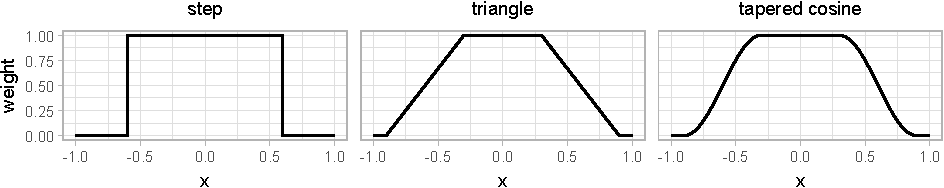
\includegraphics[width=1\linewidth]{figure_2} 

}

\caption{Weighting functions investigated in this study to make power transformations more robust against outliers. In this example, the step function was parameterised with $\delta_1 = 0.60$. The triangle and tapered cosine functions were both parameterised with $\delta_1 = 0.30$ and $\delta_2 = 0.90$.}\label{fig:weighting-functions}
\end{figure}

Each weighting function has an argument \(\dot{x}\) that is related to
the (transformed) feature in one of several ways:

\begin{itemize}
\item
  The weighting function uses empirical probabilities of the
  distribution of the original feature \(\mathbf{X}\). After sorting
  \(\mathbf{X}\) in ascending order, probabilities are determined as
  \(p_i = \frac{i - 1/3}{n + 1/3}\), with \(i = 1, 2, \ldots n\), with
  \(n\) the number of instances of feature \(\mathbf{X}\). Then
  \(\dot{x}_i = p^{*}_i=2 \left( p_i - 0.5\right)\), so that argument is
  zero-centered.
\item
  The weighting function uses the z-score of the transformed feature
  \(\phi^{\lambda, x_0, s} (\mathbf{X})\). After \citep{Raymaekers2024-zf},
  \(z_i = \frac{\phi^{\lambda, x_0, s}(x_i) - \mu_M}{\sigma_M}\). Here,
  \(\mu_M\) and \(\sigma_M\) are robust Huber M-estimates of location
  and scale of the transformed feature
  \(\phi^{\lambda, x_0, s} (\mathbf{X})\) \citep{Huber1981-su}. Then
  \(\dot{x}_i = z_i\).
\item
  After sorting \(\mathbf{X}\) in ascending order, the weighting
  function uses the residual error between the z-score of the
  transformed feature \(\phi^{\lambda, x_0, s} (\mathbf{X})\) and the
  theoretical z-score from a standard normal distribution:
  \(r_i =\left| \left( \phi^{\lambda, x_0, s}(x_i) - \mu_M)\right) / \sigma_M - F^{-1}_{\mathcal{N}}(p_i) \right|\),
  with \(\mu_M\), \(\sigma_M\) and \(p_i\) as defined above. Then
  \(\dot{x}_i = r_i\).
\end{itemize}




\subsection{Asymmetric generalised normal
distributions}\label{asymmetric-generalised-normal-distributions}

Modifications intended to make power transformations invariant to
location and scale of a feature and methods to improve their robustness
against outliers need to be assessed using data drawn from a range of
different distributions. Since the power transformations are intended
for use with unimodal distributions, the generalised normal distribution
\citep{Subbotin1923-qk, Nadarajah2005-xe} is a suitable option for simulating
realistic feature distributions. This distribution has the following
probability density function \(f_{\beta}\) for a value
\(x \in \mathbb{R}\):

\begin{definition}[Standard generalised normal distribution probability density function]
Let $x \in \mathcal{R}$.
Let $\beta > 0$ be a shape parameter.
Let $\Gamma$ be the gamma function.

Then the standard generalised normal distribution probability density function, without scale and location parameters, is:
\begin{equation}
f_{\beta}(x) = \frac{\beta}{2\Gamma\left(1 / \beta \right)} e^{-\left| x \right|^\beta}
\end{equation}
\end{definition}

For \(\beta = 1\), the probability density function describes a Laplace
distribution. A normal distribution is found for \(\beta=2\), and for
large \(\beta\), the distribution approaches a uniform distribution.

Realistic feature distributions may be skewed. Gijbels et al.~describe a
recipe for introducing skewness into the otherwise symmetric generalised
normal distribution  \citep{Gijbels2019-te}, leading to
the following probability density function:

\begin{definition}[Asymmetric generalised normal distribution probability density function]
Let $\alpha \in (0,1)$ be a skewness parameter.
Let $\mu \in \mathcal{R}$ be a location parameter.
Let $\sigma > 0$ be a shape parameter.

Then the probability density function of the asymmetric generalised normal distribution is:
\begin{equation}
f_{\alpha}(x; \mu, \sigma, \beta) = \frac{2 \alpha \left(1 - \alpha\right)}{\sigma}
\begin{cases}
f_{\beta}\left( \left(1 - \alpha \right) \frac{\left| x - \mu \right|}{\sigma} \right) & \text{, } x \leq \mu \\
f_{\beta}\left( \alpha \frac{\left| x - \mu \right|}{\sigma} \right) & \text{, } x > \mu
\end{cases}
\end{equation}
\end{definition}

\(\alpha > 0.5\) creates a distribution with a negative skew, i.e.~a
left-skewed distribution. A right-skewed distribution is created for
\(\alpha < 0.5\). \(f_{\alpha}\) thus describes the probability density
function of an asymmetric generalised normal distribution, which we will
refer to here and parametrise as
\(\mathcal{AGN}\left(\mu, \sigma, \alpha, \beta \right)\).

We require a quantile function (or an approximation thereof) to draw
random values from an asymmetric generalised normal distribution using
inverse transform sampling. Gijbels et al.~derived the quantile function
\(F_{\alpha}^{-1}(p)\), which incorporates the quantile function of the
symmetric generalised normal distribution derived by Griffin \citep{Gijbels2019-te}:

\begin{definition}[Asymmetric generalised normal distribution quantile function]
Let $p \in \left[0, 1\right]$ be a probability.
Let  $F_{\Gamma}^{-1}$ is the quantile function of the gamma distribution with shape $1 / \beta$, which can be numerically approximated. 
Let $F_{\beta}^{-1}$ be the quantile function of the generalised normal distribution:
\begin{equation}
F_{\beta}^{-1}(p) = \mathop{\mathrm{sgn}}\left(p - 0.5 \right) F_{\Gamma}^{-1}\left(2 \left|p - 0.5 \right|; 1 / \beta \right)
\end{equation}

Then the quantile function of the asymmetric generalised normal distribution is:
\begin{equation}
F_{\alpha}^{-1}(p; \mu, \sigma, \beta) =
\begin{cases}
\mu + \frac{\sigma}{1 - \alpha} F_{\beta}^{-1} \left( \frac{p}{2 \alpha}\right) & \text{, } p \leq \alpha \\
\mu + \frac{\sigma}{\alpha} F_{\beta}^{-1} \left( \frac{1 + p - 2 \alpha}{2 \left(1 - \alpha \right)} \right) & \text{, } p > \alpha
\end{cases}
\end{equation}
\end{definition}




\subsection{Central normality test}\label{central-normality-test}

Power transformations aim to transform features to a normal
distribution. However, this may not always be successful or possible.
Deviations from normality can be detected by normality tests, such as
the Shapiro-Wilk test  \citep{Gijbels2019-te}. In practice, normality
tests may be too stringent with large sample sizes, outliers, or both.
Here we develop a test for central normality.

\begin{definition}[Central portion of a sequence]
Let $\mathbf{X} = \left\{x_1, x_2, \ldots, x_n | x_i \in \mathbb{R}\right\}$ be a finite sequence of length $n > 0$,
ordered so that $x_1 \leq x_2 \leq \ldots \leq x_n$.
Let $p_i = \frac{i - 1/3}{n + 1/3}$, with $i = 1, 2, \ldots n$ be the percentile value
corresponding to each element in $\mathbf{X}$. For elements with tied values in $\mathbf{X}$,
percentile values are replaced by the average in their group, i.e.
if $x_j = x_{j+1} = \ldots = x_{j+m}$, then 
$p_j' = p_{j+1}' = \ldots = p_{j+m}' = 1/(m+1)\sum_j^{j+m}p_j$.
Furthermore, let central portion $\kappa \in (0,1)$.

Then the central portion of $\mathbf{X}$ is 
$\mathbf{X}_{\text{c}} = \left\{x_i \in \mathbf{X} \, | \,  \frac{1-\kappa}{2} \leq  p_i \leq \frac{1 + \kappa}{2}\right\}$.

\end{definition}

\begin{definition}[Residual errors of the central portion of a sequence]

Let the residual error for each element of $\mathbf{X}$ be $r_i =\left| \frac{x_i - \mu_M}{\sigma_M} - F^{-1}_{\mathcal{N}}(p_i) \right|$, 
with $\mu_M$ and $\sigma_M$ robust Huber M-estimates of location and scale of $\mathbf{X}$ \citep{Huber1981-su}, 
and $F^{-1}_{\mathcal{N}}$ the quantile function of the normal distribution $\mathcal{N}(0, 1)$.

Then, the set of residual errors of the central portion of $\mathbf{X}$ (i.e. $\mathbf{X}_{\text{c}}$) is
$\mathbf{R}_{\text{c}} = \left\{ r_i \in \left\{ r_1, r_2, \ldots, r_n\right\} \, | \,  \frac{1-\kappa}{2} \leq  p_i \leq \frac{1 + \kappa}{2}\right\}$.

\end{definition}

\begin{definition}[Central normality of a sequence]

The central portion of a sequence is normally distributed if the sum of residual
errors is equal to zero:
$\sum_{r_j \in \mathbf{R}_{\text{c}}} r_j = 0$

\end{definition}

In practice, a finite sequence sampled from a normal distribution
\(\mathcal{N}(\mu, \sigma)\) will have a non-zero sum of residual
errors.

\begin{definition}[Central normality test]
The null-hypothesis is defined as: $\mathcal{H}_0: \sum_{r_j \in \mathbf{R}_{\text{c}}}r_j = 0$

The alternative hypothesis is defined as: $\mathcal{H}_1: \sum_{r_j \in \mathbf{R}_{\text{c}}}r_j > 0$
\end{definition}

The null-hypothesis \(\mathcal{H}_0\) is that the central portion of
sequence \(\mathbf{X}\) is normally distributed, with the alternative
hypothesis \(\mathcal{H}_1\) that it is not normally distributed. To
test this hypothesis, a test statistic is computed and compared against
a critical value.

\begin{definition}[Central normality test statistic]
Let $m$ be the number of elements of $\mathbf{R}_{\text{c}}$

The test statistic is then $\tau_{n, \kappa} = \frac{1}{m}\sum_{r_j \in \mathbf{R}_{\text{c}}}r_j$.

\end{definition}

The null-hypothesis should be rejected at significance level \(\alpha\)
if \(\tau_{n, \kappa} \geq \tau_{\alpha, n, \kappa, \text{critical}}\).

The central portion of the data needs to be defined and the Type 1 error
rates determined to provide critical test statistics. We will do so in
the \hyperref[simulation]{Simulation} section.





\section{Simulation}\label{simulation}

We used simulated data to assess invariance to location and scale of the
proposed power transformations, to develop the empirical central
normality test, and to determine weighting for robust transformations.
The \(\lambda\) parameter for conventional power transformations (Eqn.
\ref{eqn:box-cox-original} and \ref{eqn:yeo-johnson-original}), as well
as \(\lambda\), \(x_0\) and \(s\) parameters for location- and
scale-invariant power transformations (Eqn. \ref{eqn:box-cox-invariant}
and \ref{eqn:yeo-johnson-invariant}) were estimated using the BOBYQA
algorithm for derivative-free bound constraint optimisation \citep{Powell2009-zb} 
through maximum likelihood estimation. The required algorithms
were implemented in the \texttt{power.transform} R software package
\citep{Zwanenburg2024-kq} (version 1.0.1). Of note, the
\texttt{power.transform} package shifts feature values into the positive
domain if negative or zero values are present for Box-Cox power
transformations.



\subsection{Invariance to location and
scale}\label{invariance-to-location-and-scale}

To assess whether the proposed power transformations lead to values of
\(\lambda\) that are invariant to location and scale of the
distribution, we simulated three different sequences. We first randomly
drew \(10000\) values from a normal distribution:
\(\mathbf{X}_{\text{normal}} = \left\{x_1, x_2, \ldots, x_{10000} \right\} \sim \mathcal{N}\left(0, 1\right)\),
or equivalently
\(\mathbf{X}_{\text{normal}} = \left\{x_1, x_2, \ldots, x_{10000} \right\} \sim \mathcal{AGN}\left(0, 1/\sqrt{2}, 0.5, 2\right)\).
The second distribution was a right-skewed generalised normal
distribution
\(\mathbf{X}_{\text{right}} = \left\{x_1, x_2, \ldots, x_{10000} \right\} \sim \mathcal{AGN}\left(0, 1/\sqrt{2}, 0.2, 2\right)\).
The third distribution was a left-skewed generalised normal distribution
\(\mathbf{X}_{\text{left}} = \left\{x_1, x_2, \ldots, x_{10000} \right\} \sim \mathcal{AGN}\left(0, 1/\sqrt{2}, 0.8, 2\right)\).
We then computed transformation parameter \(\lambda\) using the original
definitions (Eqn. \ref{eqn:box-cox-original} and
\ref{eqn:yeo-johnson-original}) and the location- and scale-invariant
definitions (Eqn. \ref{eqn:box-cox-invariant} and
\ref{eqn:yeo-johnson-invariant}) for each distribution. To assess
location invariance, a positive value \(d_{\text{shift}}\) was added to
each distribution with \(d_{\text{shift}} \in [1, 10^6]\). Similarly, to
assess scale invariance, each distribution was multiplied by a positive
value \(d_{\text{scale}}\), where \(d_{\text{scale}} \in [1, 10^6]\).

\begin{figure}

{\centering 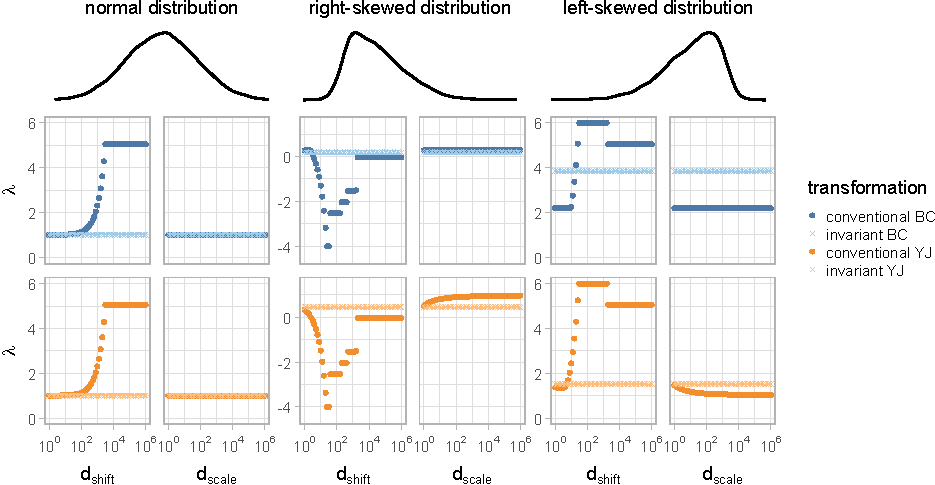
\includegraphics[width=1\linewidth]{figure_3} 

}

\caption{Invariant power transformation produces transformation parameters that are invariant to location and scale. Samples were drawn from normal, right-skewed and left-skewed distributions, respectively, which then underwent a shift $d_{\text{shift}}$ or multiplication by $d_{\text{scale}}$. Estimates of the transformation parameter $\lambda$ for the conventional power transformations show strong dependency on the overall location and scale of the distribution, whereas estimates obtained for the location- and scale-invariant power transformations are constant.}\label{fig:shifted-distributions}
\end{figure}

The result is shown in Figure \ref{fig:shifted-distributions}. For each
distribution, transformation parameter \(\lambda\) varied with
\(d_{\text{shift}}\) and \(d_{\text{scale}}\) when estimated for
conventional transformations. In contrast, estimation of \(\lambda\) for
invariant power transformations was invariant to both
\(d_{\text{shift}}\) and \(d_{\text{scale}}\).



\subsection{Central normality and empirical central normality
test}\label{central-normality-and-empirical-central-normality-test}

To develop a test for central normality we need to consider two
parameters: the central portion \(\kappa\) as a fixed parameter, and
test statistic \(\tau_{\text{ecn}}\). We will first define the central
portion \(\kappa\).

For each number of samples
\(n \in \left\{\lfloor 10^\nu \rfloor | \nu \in \left\{0.7500, 0.8125, \ldots, 4.0000 \right \} \right\}\)
we randomly drew \(m_d = 30000\) ordered sequences \(\mathbf{X}\) from
\(\mathcal{N}(0,1)\). This dataset was used to compute the critical test
statistic values for the central normality test. Additionally, we added
\(10 \%\) outliers by randomly replacing elements of each ordered
sequence. The dataset with outliers was used to compute the critical
test statistic values for the empirical variant of the central normality
test. For each sequence we then computed \(\tau_{n, \kappa}\) for
\(\kappa \in \left\{0.60, 0.70, 0.80, 0.90, 0.95, 1.00\right\}\).

Figure \ref{fig:empirical-central-normality-kappa} shows
\(\tau_{\alpha = 0.05, n, \kappa}\) as a function of \(n\) for different
values of \(\kappa\). With decreasing \(\kappa\), the test statistic
curve decreases. The curves for \(\kappa = 0.60\), \(\kappa = 0.70\) and
\(\kappa = 0.80\) are similar, whereas curves for \(\kappa \geq 0.90\)
are affected by outliers, as can be observed by comparing curves of the
central normality test with those of the empirical variant.

Since the (empirical) central normality tests assesses whether the
central part of a sequence is normally distributed, we used
\(\kappa = 0.80\). Critical statistic values for central normality and
empirical central normality tests are shown are shown in Table
\ref{tab:central-normality-critical-statistic} and Table
\ref{tab:empirical-central-normality-critical-statistic}, respectively.

\begin{figure}

{\centering 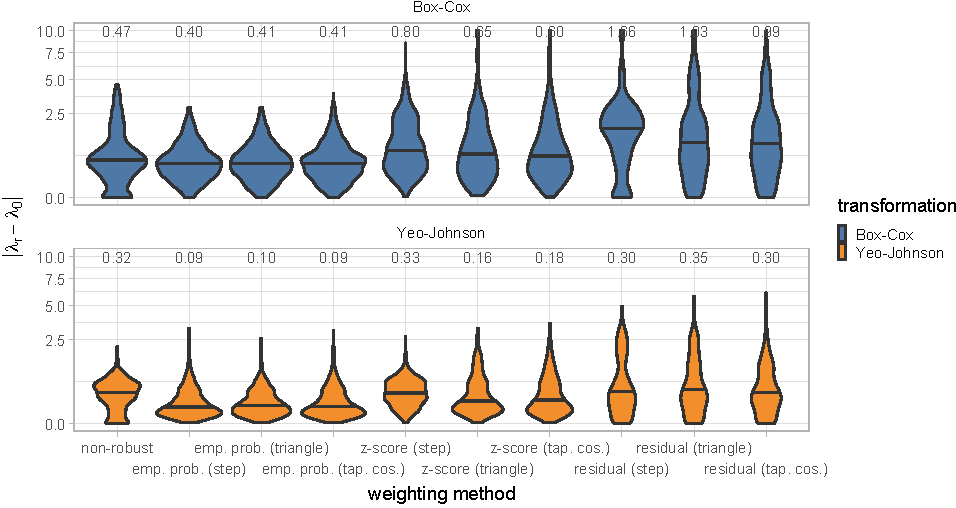
\includegraphics[width=1\linewidth]{figure_4}

}

\caption{Critical test statistic $\tau_{\alpha = 0.05, n, \kappa}$ of the (empirical) central normality test as function of $n$ for several values of central portion $\kappa$. The critical test statistics for central normality test are determined using fully normal data, whereas the statistics for the empirical variant are determined using centrally normal data, i.e. with fully normal data where 10\% of elements are replaced by outliers. emp: empirical}\label{fig:empirical-central-normality-kappa}
\end{figure}

To assess type I error rates for the (empirical) central normality test
and compare these to the Shapiro-Wilk test for normality, we randomly
drew another 1000 sequences from a standard normal distribution
(\(\mathcal{N}(0,1)\) for each
\(n \in \left\{\lfloor 10^\nu \rfloor | \nu \in \left\{0.7500, 0.8125, \ldots, 3.0000 \right \} \right\}\).
A second dataset was created by replacing elements with randomly drawn
outliers, as described above. For each sequence, the p-value for the
respective test was used to reject the null hypothesis that the sequence
is (centrally) normal. The null hypothesis was rejected if
\(p \leq 0.05\). The type I error rate was determined by computing the
fraction of centrally normal sequences rejected this way. Figure
\ref{fig:empirical-central-normality-error_rate} shows that the
empirical central normality test had the expected type I error rate for
centrally normal data (with tails of the distribution not being normally
distributed), whereas the central normality test and Shapiro-Wilk test
overestimated type I error rates.

\begin{figure}

{\centering 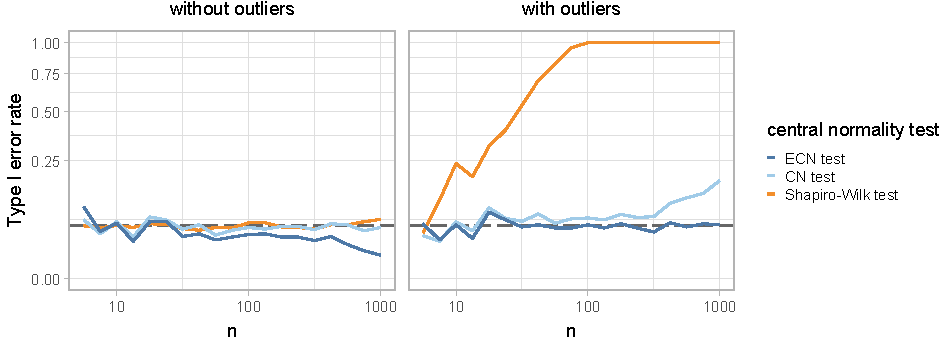
\includegraphics[width=1\linewidth]{figure_5}

}

\caption{Observed type I error rates for (central) normality tests in the presence of data derived from normal distributions with and without outliers. The empirical central normality (ECN) test uses $\kappa = 0.80$. CN: central normality}\label{fig:empirical-central-normality-error_rate}
\end{figure}

In Figure \ref{fig:empirical-central-normality-examples} we apply the
empirical central normality test to assess central normality of features
that are composed of a mixture of samples drawn from two normal
distributions (\(n = 100\) each). With increased separation of the
underlying normal distributions, the probability of the feature being
centrally normal decreases, as expected.

\begin{figure}

{\centering 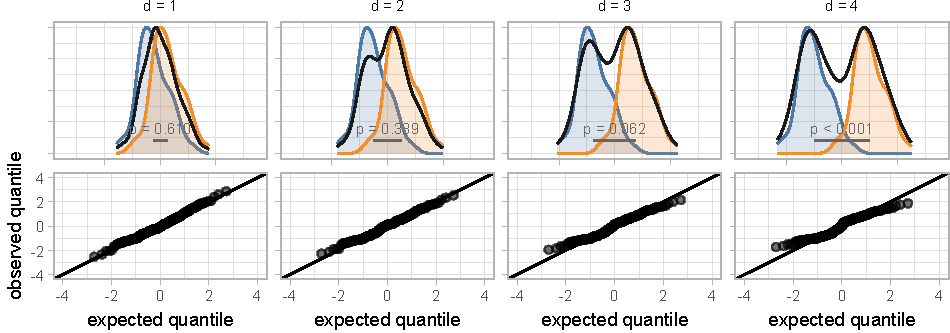
\includegraphics[width=1\linewidth]{figure_6}

}

\caption{Bi-modal distributions and empirical central normality test results. The feature (black) is a mixture of two identical sample sets (blue and orange, $n = 100$) drawn from normal distributions that are offset by a distance $d$. We use the empirical centrally normality test to compute the probability for the hypothesis that the distribution is centrally normal. As may be observed, with increasing offset $d$ the probability that the feature is centrally normal decreases. Quantile-quantile plots are drawn below each distribution.}\label{fig:empirical-central-normality-examples}
\end{figure}




\subsection{Robust transformations}\label{robust-transformations}

Outliers may be present in data and affect estimation of transformation
parameters. The log-likelihood function can be weighted to assign less
weight to outlier instances, see equations
\ref{eqn:box-cox-weighted-invariant-log-likelihood} and
\ref{eqn:yeo-johnson-weighted-invariant-log-likelihood}. We propose
three weighting functions: step, triangle and tapered cosine, that have
one, two and two parameters, respectively. Each weighting function then
uses one of the following inputs: probabilities of the empirical
distribution of the original feature, the z-score of the transformed
feature values, or the residual error between the z-score of the
transformed feature values and their expected z-score based on the
normal distribution.

To determine the weighting function parameters for each of the nine
combinations, \(m_d=500\) sequences \(\mathbf{X}_i\)
(\(i \in \{1, 2, \ldots, m_d\}\)) were randomly drawn from randomly
parametrised asymmetric generalised normal distributions. Each
distribution was parametrised with a random skewness parameter
\(\alpha \sim U\left(0.01, 0.99\right)\) and shape parameter
\(\beta \sim U\left(1.00, 5.00 \right)\). Location and scale parameters
were set as \(\mu = 0\) and \(\sigma = 1\), respectively. To form each
sequence \(\mathbf{X}_i\), \(n = \lceil 10^\gamma \rceil\) instances
were then randomly drawn, with
\(\gamma \sim U\left(\log_{10}50, 3\right)\), resulting in a set of
sequences with between \(50\) and \(1000\) elements each.

Outlier values were then drawn to randomly replace 10 percent of the
elements of \(\mathbf{X}_i\). Outlier values were set according to \citet{Tukey1977-xm},
as follows. Let \(x^{*} \sim U\left(-2, 2\right)\).
Then the corresponding outlier value was:

\begin{equation}
x_{out} =
\begin{cases}
Q_1 - \left(1.5 - x^{*} \right) \text{IQR} & \text{if } x^{*} < 0 \\
Q_3 + \left(1.5 + x^{*} \right) \text{IQR} & \text{if } x^{*} \geq 0
\end{cases}
\end{equation}

\(Q_1\), \(Q_3\) and \(\text{IQR}\) are the first quartile, third
quartile and interquartile range of \(\mathbf{X}_i\), respectively.
Outlier values randomly replaced elements in \(\mathbf{X}_i\).

To find the optimal values for the weighting function parameters
\(\delta_1\) and \(\delta_2\) (if applicable), we minimised a composite
loss
\(L = \sum_{i=1}^{m_d} L_{\text{cn},i} + 0.1 \sum_{i=1}^{m_d} L_{\lambda,i}\).
The composite loss consisted of two components: a loss term
\(L_{\text{cn},i} = \tau_{n_i, \kappa = 0.80,i}\), i.e.~the mean of
residual errors of the central 80\% of elements of each sequence
\(\mathbf{X}_i\), which aimed at optimising central normality; and a
loss term
\(L_{\lambda,i} = \max\left(0.0,|\lambda_{0,i} - \lambda_{i}| - \xi \right)\),
with \(\lambda_{0,i}\) and \(\lambda_{i}\) transformation parameters
found for sequence \(\mathbf{X}_i\) prior to and after adding outliers,
respectively, and tolerance parameter \(\xi = 0.5\) for Box-Cox and
\(\xi = 0.3\) for Yeo-Johnson power transformations. This second term
aimed to prevent solutions that provide small improvements in central
normality at the cost of a poor fit of the tails of sequences.

Minimisation was conducted using the BOBYQA algorithm for
derivative-free bound constraint optimisation \citep{Powell2009-zb}. The
resulting weighting function parameters for weighted MLE are shown in
Tables \ref{tab:optimal-weighting-parameters-box-cox} and
\ref{tab:optimal-weighting-parameters-yeo-johnson} for robust location-
and scale-invariant Box-Cox and Yeo-Johnson transformations,
respectively.

\begin{table}
\caption{Optimal weighting parameters and corresponding loss for location- and scale-invariant Box-Cox power transformations.
$p^{*}$ indicates use of the empirical distribution of feature values, $z$ the z-score of the transformed feature values,
and $r$ the residual error between the z-score of transformed feature values and the expected z-score according to the normal distribution.
The \textit{initial} column shows the starting parameter value for the optimisation process, with the corresponding boundary values in the \textit{limits} column. 
The \textit{optimal} column shows the optimal parameter values.
The \textit{loss} column shows the composite loss achieved by each method under optimised parameters.
This loss is based on residual errors of transformed features and deviations in $\lambda$ parameters
found compared to the $\lambda$ parameters found prior to inserting outliers.
The loss metric can be compared between different weighting methods.
}
\label{tab:optimal-weighting-parameters-box-cox}
\begin{tabular}{l r r r r r r r}

\toprule
method & \multicolumn{3}{c}{$\delta_1$} & \multicolumn{3}{c}{$\delta_2$} & loss \\
& initial & limits & optimal & initial & limits & optimal & \\

\midrule
non-robust               & ---  & ---       & ---  & ---  & ---       & ---  & 49.6 \\
$p^{*}$ (step)           & 0.80 & $(0, 1]$  & 0.80 & ---  & ---       & ---  & 38.5 \\
$p^{*}$ (triangle)       & 0.80 & $(0, 1]$  & 0.01 & 1.00 & $(0, 1]$  & 0.86 & 43.7 \\
$p^{*}$ (tapered cosine) & 0.80 & $(0, 1]$  & 0.00 & 1.00 & $(0, 1]$  & 0.90 & 42.7 \\
$z$ (step)               & 1.28 & $(0, 10]$ & 2.39 & ---  & ---       & ---  & 52.2 \\
$z$ (triangle)           & 1.28 & $(0, 10]$ & 2.39 & 2.40 & $(0, 10]$ & 4.92 & 52.7 \\
$z$ (tapered cosine)     & 1.28 & $(0, 10]$ & 1.07 & 3.63 & $(0, 10]$ & 3.43 & 57.4 \\
$r$ (step)               & 0.50 & $(0, 10]$ & 0.83 & ---  & ---       & ---  & 53.1 \\
$r$ (triangle)           & 0.50 & $(0, 10]$ & 0.80 & 0.81 & $(0, 10]$ & 0.84 & 54.4 \\
$r$ (tapered cosine)     & 0.50 & $(0, 10]$ & 0.76 & 0.77 & $(0, 10]$ & 0.76 & 53.2 \\
\bottomrule
\end{tabular}
\end{table}

\begin{table}
\caption{Optimal weighting parameters and corresponding loss for location- and scale-invariant Yeo-Johnson power transformations.
$p^{*}$ indicates use of the empirical distribution of feature values, $z$ the z-score of the transformed feature values,
and $r$ the residual error between the z-score of transformed feature values and the expected z-score according to the normal distribution. 
The \textit{initial} column shows the starting parameter value for the optimisation process, with the corresponding boundary values in the \textit{limits} column.
The \textit{loss} column shows the composite loss achieved by each method under optimised parameters.
This loss is based on residual errors of transformed features and deviations in $\lambda$ parameters
found compared to the $\lambda$ parameters found prior to inserting outliers.
The loss metric can be compared between different weighting methods.
}
\label{tab:optimal-weighting-parameters-yeo-johnson}
\begin{tabular}{l r r r r r r r}

\toprule
method & \multicolumn{3}{c}{$\delta_1$} & \multicolumn{3}{c}{$\delta_2$} & loss \\
& initial & limits & optimal & initial & limits & optimal & \\

\midrule
non-robust               & ---  & ---       & ---  & ---  & ---       & ---  & 42.1 \\
$p^{*}$ (step)           & 0.80 & $(0, 1]$  & 0.78 & ---  & ---       & ---  & 35.1 \\
$p^{*}$ (triangle)       & 0.80 & $(0, 1]$  & 0.20 & 0.95 & $(0, 1]$  & 1.00 & 34.0 \\
$p^{*}$ (tapered cosine) & 0.80 & $(0, 1]$  & 0.54 & 0.95 & $(0, 1]$  & 1.00 & 32.6 \\
$z$ (step)               & 1.28 & $(0, 10]$ & 2.32 & ---  & ---       & ---  & 43.0 \\
$z$ (triangle)           & 1.28 & $(0, 10]$ & 1.28 & 1.96 & $(0, 10]$ & 3.43 & 49.7 \\
$z$ (tapered cosine)     & 1.28 & $(0, 10]$ & 0.41 & 1.96 & $(0, 10]$ & 3.75 & 51.3 \\
$r$ (step)               & 0.50 & $(0, 10]$ & 0.92 & ---  & ---       & ---  & 65.4 \\
$r$ (triangle)           & 0.50 & $(0, 10]$ & 0.87 & 1.00 & $(0, 10]$ & 0.87 & 66.0 \\
$r$ (tapered cosine)     & 0.50 & $(0, 10]$ & 1.06 & 1.00 & $(0, 10]$ & 1.07 & 67.1 \\
\bottomrule
\end{tabular}
\end{table}

\subsection{Assessing transformations using simulated
data}\label{assessing-transformations-using-simulated-data}

Three datasets with 10000 sequences each were created to assess
transformation to normality. For each sequence \(\mathbf{X}_i\),
\(n = \lceil 10^\gamma \rceil\) elements were randomly drawn, with
\(\gamma \sim U\left(1, 4\right)\), resulting in sequences with between
\(10\) and \(10000\) elements.

\begin{itemize}
\item
  A \textit{clean} dataset with each sequence drawn from
  \(\mathcal{N}(0, 1)\) and transformed using an inverse power
  transformation with randomly drawn transformation parameter
  \(\lambda \sim U\left(0.00, 2.00 \right)\).
  \(\left(\phi_{\text{BC}}^\lambda\right)^{-1}\) and
  \(\left(\phi_{\text{YJ}}^\lambda\right)^{-1}\) were used as inverse
  transformations for assessing Box-Cox and Yeo-Johnson transformations,
  respectively. Prior to inverse transformation, sequences for Box-Cox
  transformations were shifted into the positive domain, with minimum
  value \(1\).
\item
  A \textit{dirty} dataset with each sequence drawn from
  \(\mathcal{AGN}\left(\mu = 0, \sigma = 1/\sqrt{2}, \alpha, \beta \right)\),
  with randomly drawn skewness parameter
  \(\alpha \sim U\left(0.01, 0.99\right)\) and shape parameter
  \(\beta \sim U\left(1.00, 5.00 \right)\).
\item
  A \textit{shifted} dataset with each sequence drawn from
  \(\mathcal{AGN}\left(\mu = 100, \sigma = 10^{-3} \cdot 1/\sqrt{2} , \alpha, \beta \right)\),
  with randomly drawn skewness parameter
  \(\alpha \sim U\left(0.01, 0.99\right)\) and shape parameter
  \(\beta \sim U\left(1.00, 5.00 \right)\).
\end{itemize}

A dataset with outliers was created for each of the above datasets by
replacing 10 percent of elements in each sequence, as described earlier.

In addition to no power transformation and location- and scale-invariant
power transformations, conventional and Raymaekers and Rousseeuw's
robust adaptation \citep{Raymaekers2024-zf} were assessed. For the
latter two methods, normalisation before standardisation using was
additionally assessed using the following two methods:

\begin{enumerate}
\def\labelenumi{\arabic{enumi}.}
\item
  z-standardisation:
  \(x^{\prime}_{i} = \left(x_i - \mu \right) / \sigma\), with \(\mu\)
  and \(\sigma\) the mean and standard deviation of sequence
  \(\mathbf{X}\).
\item
  robust scaling:
  \(x^{\prime}_{i} = \left(x_i - \text{median}\left(\mathbf{X}\right) \right) / \text{IQR}\left(\mathbf{X}\right)\),
  with \(\text{IQR}\) representing the interquartile range of
  \(\mathbf{X}\).
\end{enumerate}

This results in nine types of power transformation. Transformation
parameters were optimised for each sequence. Subsequently the sum of
residual errors and sum of residual errors of the central portion
(\(\kappa = 0.80\)) were computed for each sequence after
transformation. Then, each method was ranked according to the sum of
residual errors (data without outliers) or the sum of residual errors of
the central portion (data with outliers). The average rank of each
transformation method was computed over all 10000 sequences in each
dataset. Average ranks for Yeo-Johnson transformations are shown in
Table \ref{tab:comparison_methods_simulations_yeo_johnson}. Location and
shift-invariant Yeo-Johnson transformation ranked best for all datasets
without outliers. The robust variant ranked best in dirty and shifted
datasets with outliers, but not in the clean dataset. Results for
Box-Cox transformations are shown in Table
\ref{tab:comparison_methods_simulations_box_cox}.

\begin{table}
\caption{
Comparison of average rank between Yeo-Johnson transformation methods based on either residual error (without outliers) or residual error of the central portion
(with outliers; $\kappa = 0.80$) over 3 datasets with 10000 sequences each. The clean dataset consists of sequences derived through inverse Yeo-Johnson transformation
of data sampled from a standard normal distribution. The dirty dataset contains sequences sampled from asymmetric generalised normal distributions, centred at 0.
The shifted dataset also contains sequences sampled from asymmetric generalised normal distributions, but centred at 100, and scaled by 0.001.
Several transformation methods include normalisation before transformation, indicated by z-score normalisation (norm.) or robust scaling.
A rank of 1 is the best and a rank of 9 the worst. For each dataset, the best ranking transformation is marked in bold.
}
\label{tab:comparison_methods_simulations_yeo_johnson}
\begin{tabular}{l | l r r r r r r}

\toprule
& dataset: & \multicolumn{2}{c}{clean} & \multicolumn{2}{c}{dirty} & \multicolumn{2}{c}{shifted} \\
transformation & outliers: & no & yes & no & yes & no & yes \\

\midrule

none                                  & &         8.51  &         7.60  &         7.33  &         6.15  &         7.44  &         6.60 \\
conventional                          & &         3.70  &         5.70  &         3.87  &         7.06  &         6.49  &         5.93 \\
conventional (z-score norm.)          & &         4.72  &         5.68  &         6.38  &         5.01  &         5.43  &         4.87 \\
conventional (robust scaling)         & &         4.06  &         6.77  &         5.37  &         5.75  &         4.41  &         5.63 \\
Raymaekers-Rousseeuw                  & &         4.50  &         3.20  &         4.01  &         4.13  &         6.27  &         5.65 \\
Raymaekers-Rousseeuw (z-score norm.)  & &         5.27  & \textbf{2.66} &         6.23  &         3.59  &         5.28  &         3.48 \\
Raymaekers-Rousseeuw (robust scaling) & &         4.70  &         2.95  &         5.32  &         3.77  &         4.36  &         3.66 \\
invariant                             & & \textbf{3.13} &         6.77  & \textbf{3.22} &         6.12  & \textbf{2.64} &         6.03 \\
robust invariant                      & &         6.41  &         3.66  &         3.27  & \textbf{3.41} &         2.68  & \textbf{3.10} \\

\bottomrule
\end{tabular}
\end{table}






\section{Experimental Results}\label{experimental-results}

\subsection{Invariance}\label{invariance}

Location- and scale-invariant power transformations are intended to
yield improved transformations to normality in the presence of large
shifts in location, distributions that due to location and scale are not
centered near zero, or both. Earlier, we assessed these transformations
using simulated data. In the following, they are evaluated using
examples from real datasets. We focus on the Yeo-Johnson transformation
because of its ability to handle features with negative values. Results
for Box-Cox transformations are shown in \hyperref[appendix-e]{Appendix E}.

\begin{figure}

{\centering 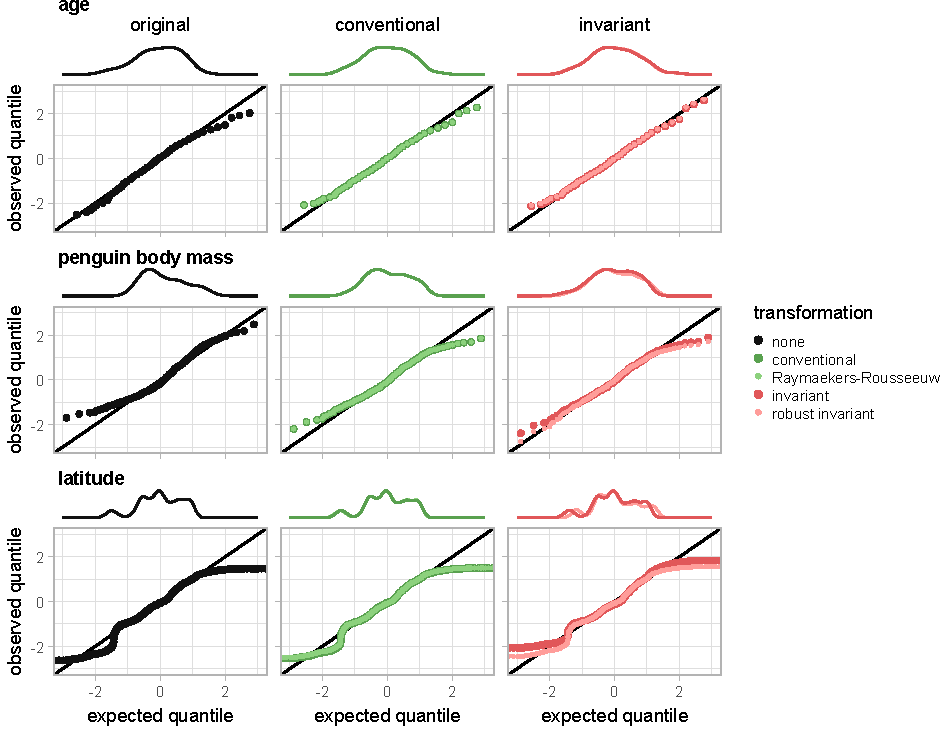
\includegraphics[width=1\linewidth]{figure_7}

}

\caption{Quantile-quantile plots for several datasets: age of patients with lung cancer (top row); penguin body mass (middle row); and latitude coordinates of houses sold in Ames, Iowa (bottom row). Multiple quantile-quantile plots are shown: for the original feature (left column); the feature transformed using the conventional Yeo-Johnson transformation and Raymaekers and Rousseeuw's robust adaptation (middle column); and the feature transformed using the non-robust and robust location- and-scale invariant Yeo-Johnson transformations (right column).}\label{fig:experimental-results-invariance}
\end{figure}

\subsubsection{Age of patients with lung
cancer}\label{age-of-patients-with-lung-cancer}

A common feature in health-related datasets is age. Here we use data on
228 patients with lung cancer that was collected and published by
Loprinzi et al. \citep{Loprinzi1994-cd}. The age in the cohort was
\(62.4 \pm 9.1\) (mean $\pm$ standard deviation) years. Applying
conventional and invariant Yeo-Johnson transformations to patient age
yielded the following results, see Figure
\ref{fig:experimental-results-invariance}: no transformation
(\(\sum r_i = 16.5\), \(p = 0.69\)); conventional transformation
(\(\lambda = 2.0\), \(\sum r_i = 11.5\), \(\mu_{YJ} = 1.8 \cdot 10^3\),
\(\sigma_{YJ} = 0.5 \cdot 10^3\), \(p = 0.96\)); Raymaekers and
Rousseeuw's robust adaptation (\(\lambda = 2.0\), \(\sum r_i = 11.5\),
\(\mu_{YJ} = 1.8 \cdot 10^3\), \(\sigma_{YJ} = 0.5 \cdot 10^3\),
\(p = 0.96\)); location- and scale-invariant transformation
(\(\lambda = 1.3\), \(\sum r_i = 8.8\), \(\mu_{YJ} = -1.2\),
\(\sigma_{YJ} = 1.1\), \(p = 0.98\)); and robust location- and
scale-invariant transformation (\(\lambda = 1.3\), \(\sum r_i = 9.3\),
\(\mu_{YJ} = -1.0\), \(\sigma_{YJ} = 1.1\), \(p = 0.93\)).

Location- and scale-invariant transformation led to a lower overall
residual error, indicating a better transformation to normality.
Conventional transformations inflated the mean \(\mu_{YJ}\) and standard
deviation \(\sigma_{YJ}\) of the age feature after transformation. The
empirical central normality test did not detect any statistically
significant deviations from central normality for any transformation
(all \(p \geq 0.93\)).

\subsubsection{Penguin body mass}\label{penguin-body-mass}

Gorman, Williams and Fraser recorded body mass (in grams) of 342
penguins of three different species \citep{Gorman2014-eo}.
The body mass was \((4.2 \pm 0.8) \cdot 10^3\) (mean $\pm$ standard
deviation) grams, and not centrally normal (\(p < 0.001\)). Applying
conventional and invariant Yeo-Johnson transformations to body mass
yielded the following results, see Figure
\ref{fig:experimental-results-invariance}: no transformation (residual
sum \(\sum r_i = 48.0\), \(p < 0.001\)); conventional transformation
(\(\lambda = -0.5\), \(\sum r_i = 32.2\), \(\mu_{YJ} = 2.1\),
\(\sigma_{YJ} = 4 \cdot 10^{-3}\), \(p = 0.10\)); Raymaekers and
Rousseeuw's robust adaptation (\(\lambda = -0.5\), \(\sum r_i = 32.2\),
\(\mu_{YJ} = 2.1\), \(\sigma_{YJ} = 4 \cdot 10^{-3}\), \(p = 0.10\));
location- and scale-invariant transformation (\(\lambda = 0.5\),
\(\sum r_i = 26.8\), \(\mu_{YJ} = 0.9\), \(\sigma_{YJ} = 0.9\),
\(p = 0.28\)); and robust location- and scale-invariant transformation
(\(\lambda = 0.3\), \(\sum r_i = 22.0\), \(\mu_{YJ} = 0.7\),
\(\sigma_{YJ} = 0.9\), \(p = 0.69\)).

Location- and scale-invariant transformation produced a lower overall
residual errors, indicating a better transformation. Moreover,
conventional transformations led to low standard deviation
\(\sigma_{YJ}\) of the body mass feature after transformation. The
empirical central normality test did not detect any statistically
significant deviations from central normality for any transformation
(all \(p \geq 0.10\)).

\subsubsection{Latitude in the Ames housing
dataset}\label{latitude-in-the-ames-housing-dataset}

Geospatial datasets usually contain coordinates. The Ames housing
dataset contains data on 2930 properties that were sold between 2006 and
2010 \citep{De-Cock2011-jf}, including their geospatial coordinates. The
latitude was \(42.03 \pm 0.02)\) (mean $\pm$ standard deviation). Applying
conventional and invariant Yeo-Johnson transformations to latitude
yielded the following results, see Figure
\ref{fig:experimental-results-invariance}: no transformation (residual
sum \(\sum r_i = 328\), \(p < 0.001\)); conventional transformation
(\(\lambda = 62.1\), \(\sum r_i = 319\),
\(\mu_{YJ} = 4.8 \cdot 10^{99}\), \(\sigma_{YJ} = 0.1 \cdot 10^{99}\),
\(p < 0.001\)); Raymaekers and Rousseeuw's robust adaptation
(\(\lambda = 95.4\), \(\sum r_i = 315\),
\(\mu_{YJ} = 6.4 \cdot 10^{153}\), \(\sigma_{YJ} = 0.3 \cdot 10^{153}\),
\(p < 0.001\)); location- and scale-invariant transformation
(\(\lambda = 1.5\), \(\sum r_i = 326\), \(\mu_{YJ} = -1.2\),
\(\sigma_{YJ} = 0.8\), \(p < 0.001\)); and robust location- and
scale-invariant transformation (\(\lambda = 1.1\), \(\sum r_i = 308\),
\(\mu_{YJ} = -1.3\), \(\sigma_{YJ} = 1.2\), \(p < 0.001\)).

Every transformation reduced the residual sum. None of the
transformations yielded a centrally normal distribution. Conventional
transformations had high values for the \(\lambda\) parameter, which
could lead to numerical issues.



\subsection{Robustness against
outliers}\label{robustness-against-outliers}

We previously simulated data to assess invariant power transformations
and their robustness against outliers. Here, we assess invariant power
transformations in real data with outliers.

\begin{figure}

{\centering 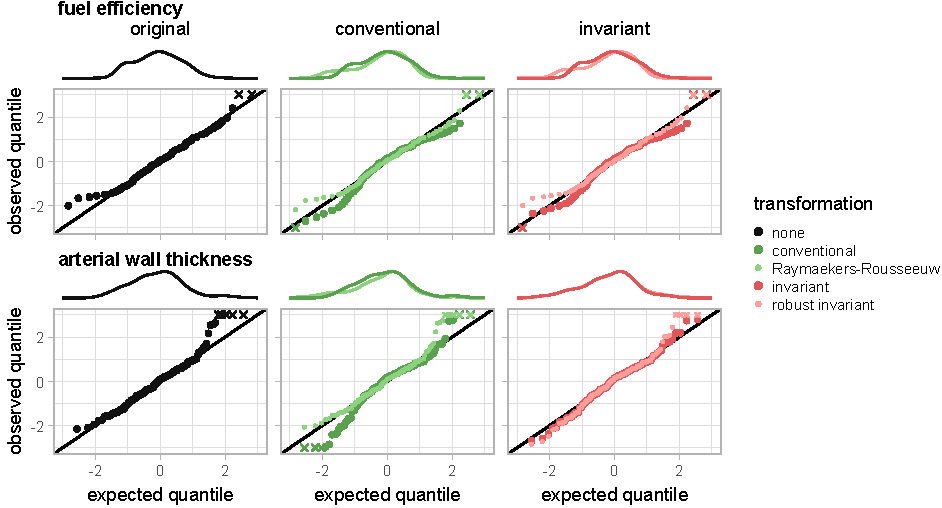
\includegraphics[width=1\linewidth]{figure_8}

}

\caption{Quantile-quantile plots for two datasets with outliers: vehicle fuel consumption (top row), where outliers are related to highly fuel-efficient vehicles; and maximum arterial wall thickness in patients with ischemic stroke (bottom row). Multiple quantile-quantile plots are shown: for the original feature (left column); the feature transformed using the conventional Yeo-Johnson transformation and Raymaekers and Rousseeuw's robust adaptation (middle column); and the feature transformed using the non-robust and robust location- and-scale invariant Yeo-Johnson transformations (right column). Samples with observed quantiles below $-3.0$ or above $3.0$ are indicated by crosses.}\label{fig:experimental-results-outlier-robustness}
\end{figure}

\subsubsection{Fuel efficiency in the Top Gear
dataset}\label{fuel-efficiency-in-the-top-gear-dataset}

The Top Gear dataset contains data on 297 vehicles that appeared on the
BBC television show \emph{Top Gear} \citep{Alfons2021-kc}. Within this dataset,
the fuel consumption feature contains outliers due to highly
fuel-efficient vehicles. Applying conventional and invariant Yeo-Johnson
transformations to the fuel consumption feature yielded the following
results, see Figure \ref{fig:experimental-results-outlier-robustness}:
no transformation (residual sum \(\sum r_i = 54\), \(p=0.72\));
conventional transformation (\(\lambda = -0.1\), \(\sum r_i = 55\),
\(\mu_{YJ} = 3.0\), \(\sigma_{YJ} = 0.3\), \(p < 0.001\)); Raymaekers
and Rousseeuw's robust adaptation (\(\lambda = 0.8\), \(\sum r_i = 48\),
\(\mu_{YJ} = 29\), \(\sigma_{YJ} = 15\), \(p=0.37\)); location- and
scale-invariant transformation (\(\lambda = -1.3\), \(\sum r_i = 44\),
\(\mu_{YJ} = 0.5\), \(\sigma_{YJ} = 0.1\), \(p < 0.001\)); and robust
location- and scale-invariant transformation (\(\lambda = 1.0\),
\(\sum r_i = 56\), \(\mu_{YJ} = 1.7\), \(\sigma_{YJ} = 1.0\),
\(p=0.76\)).

Outliers cause non-robust transformations to fail to transform the data
to a centrally normal distribution (empirical central normality test
\(p < 0.001\) for conventional and invariant transformations). Robust
transformations produce distributions that are centrally normal
(empirical central normality test \(p > 0.05\)).

\subsubsection{Maximum arterial wall thickness in an ischemic stroke
dataset}\label{maximum-arterial-wall-thickness-in-an-ischemic-stroke-dataset}

The ischemic stroke dataset contains historic data from 126 patients
with risk at ischemic stroke \citep{Kuhn2019-kt}. These patients
underwent Computed Tomography Angiography to characterize the carotid
artery blockages. Angiography imaging was then assessed, and various
characteristics related to the blood vessels and the disease are
measured. The maximum arterial wall thickness feature contains several
instances with outlier values. Applying conventional and invariant
Yeo-Johnson transformations to this feature yielded the following
results, see Figure \ref{fig:experimental-results-outlier-robustness}:
no transformation (residual sum \(\sum r_i = 110\), \(p=0.83\));
conventional transformation (\(\lambda = -0.7\), \(\sum r_i = 30\),
\(\mu_{YJ} = 1.0\), \(\sigma_{YJ} = 0.1\), \(p=0.003\)); Raymaekers and
Rousseeuw's robust adaptation (\(\lambda = 1.1\), \(\sum r_i = 136\),
\(\mu_{YJ} = 7.2\), \(\sigma_{YJ} = 14.3\), \(p=0.88\)); location- and
scale-invariant transformation (\(\lambda = 0.2\), \(\sum r_i = 12\),
\(\mu_{YJ} = -11.8\), \(\sigma_{YJ} = 6.9\), \(p=0.15\)); and robust
location- and scale-invariant transformation (\(\lambda = -0.3\),
\(\sum r_i = 30\), \(\mu_{YJ} = 0.8\), \(\sigma_{YJ} = 0.2\),
\(p=0.18\)).

The conventional non-robust transformation failed to produce a centrally
normal distribution (empirical central normality test \(p=0.003\)).
Robust transformations produce distributions that are centrally normal
(empirical central normality test \(p > 0.05\)).

\subsection{Integration into end-to-end machine
learning}\label{integration-into-end-to-end-machine-learning}

We used 231 datasets containing at least one numeric feature from the
Penn Machine Learning Benchmarks collection \citep{Romano2022-gq}. In
this collection, 114 datasets correspond to regression tasks and 117
datasets to classification tasks. Using the familiar auto-machine
learning library \citep{Zwanenburg2021-so} (version 1.5.0), each
dataset was used to train a model for each of 32 process configurations.
Each process configuration specifies the learner (generalised linear
model, L1-regularised linear models (Lasso), gradient boosted linear
model, or random forest), transformation method (none, conventional
Yeo-Johnson, robust invariant Yeo-Johnson, robust invariant Yeo-Johnson
with empirical central normality test (rejecting transformations with
\(p \leq 0.01\)), and normalisation method (none,
\(z\)-standardisation), yielding 32 distinct configurations. Before each
experiment, each dataset was randomly split into a training (70\%) and
holdout test (30\%) set five times. Thus, a total of 36960 models were
created. Each model was then evaluated using the holdout test set using
one of two metrics, i.e.~the root relative squared error (RRSE) for
regression tasks and the area under the receiver operating
characteristic curve (AUC) for classification tasks.

For the purpose of assessing the effect of the difficulty of the task,
we computed the median performance score over all models for each
dataset and assigned one the following categories:

\begin{itemize}
\item
  very easy: \(\text{AUC} \geq 0.90\) or \(\text{RRSE} \leq 0.10\) (57
  datasets)
\item
  easy: \(0.90 > \text{AUC} \geq 0.80\) or
  \(0.30 \geq \text{RRSE} > 0.10\) (40 datasets)
\item
  intermediate: \(0.80 > \text{AUC} \geq 0.70\) or
  \(0.60 \geq \text{RRSE} > 0.30\) (52 datasets)
\item
  difficult: \(0.70 > \text{AUC} \geq 0.60\) or
  \(0.80 \geq \text{RRSE} > 0.60\) (33 datasets)
\item
  very difficult: \(0.60 > \text{AUC} \geq 0.50\) or
  \(1.00 \geq \text{RRSE} > 0.80\) (48 datasets)
\item
  unsolvable: \(\text{AUC} < 0.50\) or \(\text{RRSE} > 1.00\) (1
  dataset)
\end{itemize}

To remove the effect of the dataset, and allow for comparing metrics, we
ranked all performance scores for each dataset so that a higher rank
corresponds to better performance. Experiments yielding the same score
received the same, average, rank. Subsequently ranks were normalised to
the \([0.0, 1.0]\) range.

Significant differences exist between process configurations (Friedman
test: \(p < 10^{-8})\).

Considering single process parameters, the choice of learner (Friedman
test: \(p < 10^{-8})\)), normalisation method (Wilcoxon signed rank
test: \(p = 4 \cdot 10^{-8}\)), and transformation method (Friedman
test: \(p = 0.007\)), all had a significant impact (at \(p = 0.05\)).

To estimate the marginal effects of process parameters, including
transformation method, we first fit a regression random forest (ranger
package \citep{Wright2017-rf} version 0.16.0): 2000 trees, node size
2, other hyperparameters default) with process parameters and task
difficulty as predictors and normalised rank as response variable. The
estimated marginal effects are shown in Figure
\ref{fig:marginal-effect-plot}. On the scale of normalised ranks
(\([0.0, 1.0]\)), only the random forest performed better than the
average of all learners (rank difference \(0.173\)). The marginal
improvement in performance from z-standardisation was \(0.011\).
Transformation methods had the following marginal effects: \(-0.001\)
for using conventional Yeo-Johnson transformation instead of no
transformation; \(-0.012\) for using robust invariant Yeo-Johnson
transformation instead of no transformation; \(-0.012\) for using robust
invariant Yeo-Johnson transformation with empirical central normality
test instead of no transformation; \(-0.012\) for using robust invariant
Yeo-Johnson transformation instead of conventional Yeo-Johnson
transformation; and \(-0.012\) for using using robust invariant
Yeo-Johnson transformation with empirical central normality test instead
of conventional Yeo-Johnson transformation.

\begin{figure}

{\centering 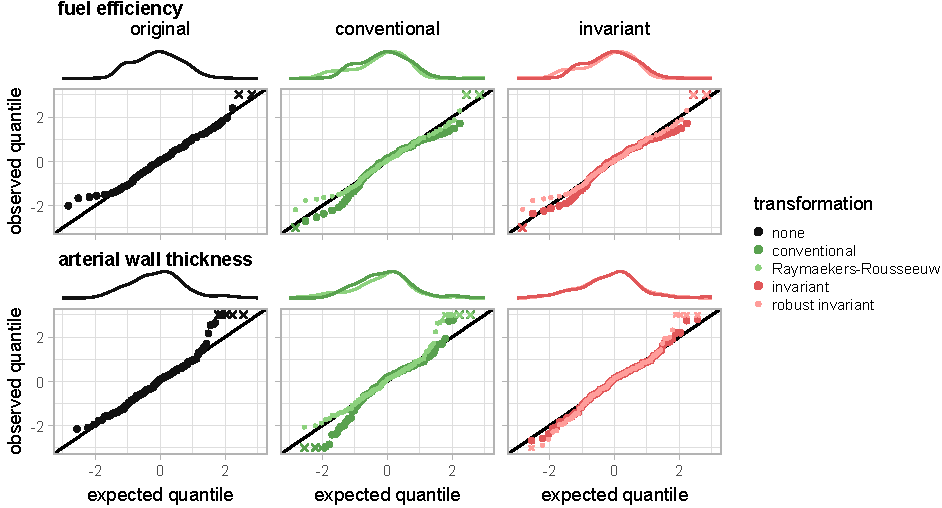
\includegraphics[width=1\linewidth]{figure_9}

}

\caption{Estimated marginal effect of learners, normalisation and transformation methods on ranked model performance scores in 36960 machine learning experiments on 231 datasets. The four top-left panels shows the marginal effect of learners vs. the average, i.e. generalised linear models (GLM), L1-regularised LM (Lasso), gradient-boosted LM and random forest. Random forests outperform the average. The top-right panel shows the marginal effect of feature normalisation methods, i.e. no normalisation and z-standardisation. z-standardisation is generally beneficial, but the estimated effect is marginal. The bottom panel shows the marginal effects of different transformation methods, split by normalisation method. The estimated effects are similar in size to the effect of normalisation and marginal. Note that the ranges of the $x$-axes of the three main panels differ. ECNT: empirical central normality test.}\label{fig:marginal-effect-plot}
\end{figure}

\FloatBarrier


\section{Discussion}\label{discussion}

In their work on power transformation, Box and Cox already mention
transformation with a shift parameter, but preferred the version in Eq.
\ref{eqn:box-cox-original} for the theoretical analysis in their paper
\citep{Box1964-mz}, which subsequently became the convention. Yeo and
Johnson's power transformation lacks a shift parameter altogether \citep{Yeo2000-vw}.
We showed that these power transformations are
sensitive to location and scale of data distributions. To mitigate this
issue, we defined location- and scale-invariant variants of the Box-Cox
and Yeo-Johnson transformations. We furthermore assessed methods for
making these transformations robust to outliers, and devised an
empirical test for central normality.

Robust location- and scale-invariant transformations are a suitable
replacement for their conventional counterparts. They demonstrated
robustness against outliers and prevent inaccurate transformations and
potential numerical issues due to location and scale of the distribution
of a feature. This is particularly relevant for automated data
processing, where such issues may go unnoticed.

In simulation, robust location- and scale-invariant transformations
ranked best in datasets with outliers, and ranked highly in datasets
without outliers, except for features without outliers that were
directly sampled from strictly normal distributions. In real-world
examples, robust location-and scale-invariant transformations achieved
central normality when the non-robust variant could not.

However, in a machine learning experiment of 231 real-world datasets
that contained at least one numeric feature, we did not find a
meaningful benefit -- nor detriment -- to model performance for
location- and scale-invariant power transformations. One reason may be
that numeric features with large location shifts (\(|\mu| > 1000.0\))
were uncommon. Of the 4886 numeric features in the 231 datasets, 266
(5\%) features in 34 datasets had large location shifts, of which 200
appeared in just 2 datasets. For the latter two datasets, the
transformation method did not show significant difference between groups
(Friedman test; \(p > 0.05\)).

Location- and scale-invariant transformations are realised by
simultaneously optimising three parameters, i.e.~transformation
parameter \(\lambda\), shift parameter \(x_0\) and scale parameter
\(s\). We derived the log-likelihood function to facilitate optimisation
using MLE. Alternatively, standardisation of a numeric feature (e.g.,
through subtracting its median value and division by its interquartile
range) prior to conventional power transformations can achieve a similar
effect in reducing sensitivity to the feature's location and scale.
While this alternative helps prevent these issues -- provided that
standardisation does not lead to negative values for Box-Cox
transformations -- location- and scale-invariant transformations are
able to achieve better transformations to normality, as demonstrated by
lower residual errors in simulation experiments.

We assessed several weighting methods to achieve robust power
transformations. Robust power transformations should satisfy two
conflicting aims: they should minimise residual errors after
transformation to central normality, and minimise the overall effect of
outliers on estimation of transformation parameter \(\lambda\). These
aims are reflected in the composite loss used to optimise weighting
parameters. For Yeo-Johnson transformation, empirical probabilities with
tapered cosine weighting resulted in the lowest loss. The optimal
parameters led to weights that gradually decline towards the tails of
empirical probabilities, i.e.~elements with low and high values receive
less or no weight. Similarly, for Box-Cox transformation, empirical
probabilities with step weighting resulted in the lowest loss. In this
case the central 80\% of the elements are used, and the remaining 10\%
in each tail are ignored. Methods that relied on the z-score of the
transformed feature or the residual error yielded worse loss than the
non-robust method or those based on empirical probabilities.
Underperformance of these weighting methods could be explained by their
reliance on transformed feature values for setting weights.
Consequently, their weights change at each iteration in the MLE
optimisation process. This increases local variance in the
log-likelihood function and creates local optima that the optimiser may
not handle well. Methods that relied on the empirical probability did
not suffer from this issue, as weights remained fixed during MLE.

We introduced an empirical test for central normality to assess whether
sequences deviate from normality in a way that might require closer
inspection prior to further processing. The empirical test for central
normality differs from other tests for normality, such as the
Shapiro-Wilk test \citep{Shapiro1965-zd}, as it assesses normality of
the central portion of a feature, instead of the entire feature.
Compared to the central normality test and the Shapiro-Wilk test, the
empirical central normality test remains consistent in the presence of
outliers, although the former tests are more powerful when outliers are
absent.

This work has the following limitation: We observed several numerical
stability issues for optimisation criteria other than MLE (\hyperref[appendix-b]{Appendix B}).
These appear in regions where transformation parameters would lead to
very large or small numbers when using conventional power
transformations. For MLE stability issues were not observed.

\section{Conclusion}\label{conclusion}

Compared to their conventional versions, robust location- and
scale-invariant Box-Cox and Yeo-Johnson transformations reduce
sensitivity to outliers and the location and scale of features. An
empirical central normality test can assess the quality of
transformation of features to normal distributions. The combination of
both facilitate the use of power transformations in automated data
analysis workflows.

\backmatter

\section*{Declarations}

\begin{itemize}
\item Funding: No funding was received for conducting this study.
\item Competing interests: The authors have no relevant financial or non-financial interests to disclose.
\item Ethics approval and consent to participate: Not applicable
\item Consent for publication: Not applicable
\item Data availability: Data and results for the machine learning experiment are available
from Zenodo (https://doi.org/10.5281/zenodo.14986689). The manuscript was created using R Markdown with integrated code and is
available from the \texttt{power.transform} GitHub repository, together with intermediate analysis results
for computationally intensive experiments.
\item Materials availability: Not applicable
\item Code availability: Location- and scale-invariant power transformations were implemented in
the \texttt{power.transform} package for R, which is available from
GitHub (https://github.com/oncoray/power.transform) and the CRAN
repository (https://cran.r-project.org/package=power.transform). The manuscript was created using R Markdown with integrated code, and is available from the \texttt{power.transform} GitHub repository.
\item Author contribution: Conceptualization: Alex Zwanenburg, Steffen L{\"o}ck; Methodology: Alex Zwanenburg; Formal analysis and investigation: Alex Zwanenburg; Writing - original draft preparation: Alex Zwanenburg; Writing - review and editing: Alex Zwanenburg, Steffen L{\"o}ck; Resources: Alex Zwanenburg, Steffen L{\"o}ck; Supervision: Steffen L{\"o}ck.
\end{itemize}






\begin{appendices}

\section{Log-likelihood functions for location- and
scale-invariant power
transformation}\label{appendix-a}

Location- and scale-invariant Box-Cox and Yeo-Johnson transformations
are parametrised using location \(x_0\) and scale \(s\) parameters, in
addition to transformation parameter \(\lambda\). This leads to the
following transformations. The location- and scale-invariant Box-Cox
transformation is:

\begin{equation}
\phi_{\text{BC}}^{\lambda, x_0, s} (x_i) = 
\begin{cases}
\left( \left(\frac{x_i - x_0}{s} \right)^\lambda - 1 \right) / \lambda & \text{if } \lambda \neq 0\\
\log\left[\frac{x_i - x_0}{s}\right] & \text{if } \lambda = 0
\end{cases}
\end{equation}

where \(x_i - x_0 > 0\). The location- and scale-invariant Yeo-Johnson
transformation is:

\begin{equation}
\phi_{\text{YJ}}^{\lambda, x_0, s} (x_i) = 
\begin{cases}
\left( \left( 1 + \frac{x_i - x_0}{s}\right)^\lambda - 1\right) / \lambda & \text{if } \lambda \neq 0 \text{ and } x_i - x_0 \geq 0\\
\log\left[1 + \frac{x_i - x_0}{s}\right] & \text{if } \lambda = 0 \text{ and } x_i - x_0 \geq 0\\
-\left( \left( 1 - \frac{x_i - x_0}{s}\right)^{2 - \lambda} - 1 \right) / \left(2 - \lambda \right) & \text{if } \lambda \neq 2 \text{ and } x_i - x_0 < 0\\
-\log\left[1 - \frac{x_i - x_0}{s}\right] & \text{if } \lambda = 2 \text{ and } x_i - x_0 < 0
\end{cases}
\end{equation}

The parameters of these power transformations can be optimised based by
maximising the log-likelihood function, under the assumption that the
transformed feature \(\phi^{\lambda, x_0, s} (\mathbf{X})\) follows a
normal distribution. The log-likelihood functions for conventional
Box-Cox and Yeo-Johnson transformations are well-known. However, the
introduction of scaling parameter \(s\) prevents their direct use. Here,
we first derive the general form of the log-likelihood functions, and
then derive their power-transformation specific definitions.

Let \(f(x_1, \ldots, x_n)\) be the probability density function of
feature \(\mathbf{X} = \{ x_1, \ldots, x_n\}\), and
\(f^{\lambda, x_0, s} (\phi^{\lambda, x_0, s}(x_1), \ldots, \phi^{\lambda, x_0, s}(x_n))\)
be the probability density function of the transformed feature
\(\phi^{\lambda, x_0, s} (\mathbf{X})\), that is assumed to follow a
normal distribution.

The two probability density functions are related as follows:

\begin{equation}
f^{\lambda, x_0, s}(x_1, \ldots, x_n) = f^{\lambda, x_0, s} (\phi^{\lambda, x_0, s}(x_1), \ldots, \phi^{\lambda, x_0, s}(x_n)) \left|\mathbf{J}\right|
\end{equation}

Where, \(\left|\mathbf{J}\right|\) is the determinant of Jacobian
\(\mathbf{J}\). The Jacobian takes the following form, with off-diagonal
elements \(0\):

\begin{equation}
\mathbf{J} =
\begin{bmatrix}
    \frac{\partial}{\partial x_1} \phi^{\lambda, x_0, s}(x_1) & 0 & \dots & 0 \\
    0 & \frac{\partial}{\partial x_2} \phi^{\lambda, x_0, s}(x_2) & \dots & 0 \\
    \vdots & \vdots  & \ddots &  \vdots \\
    0  & 0 & 0 & \frac{\partial}{\partial x_n} \phi^{\lambda, x_0, s}(x_n)
\end{bmatrix}
\end{equation}

Thus,
\(\left| \mathbf{J} \right| = \prod_{i=1}^n \frac{\partial}{\partial x_i} \phi^{\lambda, x_0, s}(x_i)\).

Since in our situation \(\{x_1, \ldots, x_n\}\) in
\(f^{\lambda, x_0, s}(x_1, \ldots, x_n)\) are considered fixed (i.e.,
known), \(f^{\lambda, x_0, s}(x_1, \ldots, x_n)\) may be considered a
likelihood function. The log-likelihood function
\(\mathcal{L}^{\lambda, x_0, s}\) is then:

\begin{equation}
\begin{split}
\mathcal{L}^{\lambda, x_0, s} & = \log f^{\lambda, x_0, s}(x_1, \ldots, x_n) \\
 & = \log \left[ f^{\lambda, x_0, s} (\phi^{\lambda, x_0, s}(x_1), \ldots, \phi^{\lambda, x_0, s}(x_n)) \right] + \log \left|\mathbf{J}\right| \\
 & = \log \left[ f^{\lambda, x_0, s} (\phi^{\lambda, x_0, s}(x_1), \ldots, \phi^{\lambda, x_0, s}(x_n)) \right] + \log \prod_{i=1}^n \frac{\partial}{\partial x_i} \phi^{\lambda, x_0, s}(x_i) \\
 & = -\frac{n}{2} \log \left[2 \pi \sigma^2 \right] -\frac{1}{2 \sigma^2} \sum_{i=1}^n \left( \phi^{\lambda, x_0, s}(x_i) - \mu \right)^2 + \sum_{i=1}^n \log \left[ \frac{\partial}{\partial x_i} \phi^{\lambda, x_0, s}(x_i)\right]
\end{split}
\end{equation}

With \(\mu\) the average of \(\phi^{\lambda, x_0, s}(\mathbf{X})\) and
\(\sigma^2\) its variance. The first two terms derive directly from the
log-likelihood function of a normal distribution, and are not specific
to the type of power transformation used. However, the final term
differs between Box-Cox and Yeo-Johnson transformations.



\subsection{Location- and scale-invariant Box-Cox
transformation}\label{location--and-scale-invariant-box-cox-transformation-appendix}

For the location- and scale-invariant Box-Cox transformation the partial
derivative is:

\begin{equation}
\begin{split}
\frac{\partial}{\partial x_i} \phi_{\text{BC}}^{\lambda, x_0, s}(x_i) & = \frac{1}{s} \left(\frac{x_i - x_0}{s} \right)^{\lambda-1} \\
 & = \frac{1} {s^\lambda} \left(x_i - x_0 \right)^{\lambda - 1}
\end{split}
\end{equation}

Thus the final term in \(\mathcal{L}_{\text{BC}}^{\lambda, x_0, s}\) is:

\begin{equation}
\begin{split}
\sum_{i=1}^n \log \frac{\partial}{\partial x_i} \phi_{\text{BC}}^{\lambda, x_0, s}(x_i) & = \sum_{i=1}^n \log \left[ s^{-\lambda} (x_i - x_0)^{\lambda - 1} \right] \\
& = \sum_{i=1}^n \log \left[s^{-\lambda} \right] + \log \left[ (x_i - x_0)^{\lambda - 1} \right]\\
& = -n \lambda \log s + \left( \lambda - 1 \right) \sum_{i=1}^n \log \left[ x_i - x_0 \right]
\end{split}
\end{equation}

This leads to the following log-likelihood:

\begin{equation}
\begin{split}
\mathcal{L}_{\text{BC}}^{\lambda, x_0, s} = & -\frac{n}{2} \log \left[2 \pi \sigma^2 \right] -\frac{1}{2 \sigma^2} \sum_{i=1}^n \left( \phi^{\lambda, x_0, s}(x_i) - \mu \right)^2 \\
& -n \lambda \log s + \left( \lambda - 1 \right) \sum_{i=1}^n \log \left[ x_i - x_0 \right]
\end{split}
\end{equation}

Similarly to \citet{Raymaekers2024-zf}, sample weights \(w_i\) are
introduced to facilitate robust power transformations. The weighted
log-likelihood of the location- and scale-invariant Box-Cox
transformation is:

\begin{equation}
\begin{split}
\mathcal{L}_{\text{rBC}}^{\lambda, x_0, s} = & -\frac{1}{2} \left(\sum_{i=1}^n w_i \right) \log \left[ 2 \pi \sigma_w^2 \right] -\frac{1}{2 \sigma_w^2} \sum_{i=1}^n w_i \left( \phi^{\lambda, x_0, s}(x_i) - \mu_w \right)^2 \\
& - \lambda \left( \sum_{i=1}^n w_i \right) \log s + \left( \lambda - 1 \right) \sum_{i=1}^n w_i \log \left[ x_i - x_0 \right]
\end{split}
\end{equation}

where \(\mu_w\) and \(\sigma^2_w\) are the weighted mean and weighted
variance of the Box-Cox transformed feature
\(\phi_{\text{BC}}^{\lambda, x_0, s} (\mathbf{X})\), respectively:

\begin{equation}
\sigma_w^2 = \frac{\sum_{i=1}^n w_i \left(\phi_{\text{BC}}^{\lambda, x_0, s} (x_i) - \mu_w \right)^2}{\sum_{i=1}^n w_i} \quad \text{with } \mu_w = \frac{\sum_{i=1}^n \phi_{\text{BC}}^{\lambda, x_0, s} (x_i)} {\sum_{i=1}^n w_i}
\end{equation}



\subsection{Location- and scale-invariant Yeo-Johnson
transformation}\label{location--and-scale-invariant-yeo-johnson-transformation-appendix}

For the location- and scale-invariant Yeo-Johnson transformation, the
partial derivative is:

\begin{equation}
\frac{\partial}{\partial x_i} \phi_{\text{YJ}}^{\lambda, x_0, s}(x_i) =
\begin{cases}
\frac{1}{s} \left(1 + \frac{x_i - x_0}{s}\right)^{\lambda - 1} & \text{if } x_i - x_0 \geq 0\\
\frac{1}{s} \left(1 - \frac{x_i - x_0}{s}\right)^{1 - \lambda} & \text{if } x_i - x_0 < 0
\end{cases}
\end{equation}

Thus the final term in \(\mathcal{L}_{\text{YJ}}^{\lambda, x_0, s}\) is:

\begin{equation}
\begin{split}
\sum_{i=1}^n \log \frac{\partial}{\partial x_i} \phi_{\text{YJ}}^{\lambda, x_0, s}(x_i) & = - n \log s + (\lambda - 1) \sum_{i=1}^n \sgn(x_i - x_0) \log \left[1 + \frac{|x_i - x_0|}{s} \right]
\end{split}
\end{equation}

This leads to the following log-likelihood:

\begin{equation}
\begin{split}
\mathcal{L}_{\text{YJ}}^{\lambda, x_0, s} = & -\frac{n}{2} \log\left[2 \pi \sigma^2\right] -\frac{1}{2 \sigma^2} \sum_{i=1}^n \left( \phi^{\lambda, x_0, s}(x_i) - \mu \right)^2 \\
& - n \log s + (\lambda - 1) \sum_{i=1}^n \sgn(x_i - x_0) \log \left[1 + \frac{|x_i - x_0|}{s} \right]
\end{split}
\end{equation}

The weighted log-likelihood for location- and scale-invariant
Yeo-Johnson transformation is:

\begin{equation}
\begin{split}
\mathcal{L}_{\text{rYJ}}^{\lambda, x_0, s} = & -\frac{1}{2} \left(\sum_{i=1}^n w_i \right) \log \left[ 2 \pi \sigma_w^2 \right] -\frac{1}{2 \sigma_w^2} \sum_{i=1}^n w_i \left( \phi^{\lambda, x_0, s}(x_i) - \mu_w \right)^2 \\
& - \left( \sum_{i=1}^n w_i \right) \log s + (\lambda - 1) \sum_{i=1}^n w_i \sgn(x_i - x_0) \log \left[1 + \frac{|x_i - x_0|}{s} \right]
\end{split}
\end{equation}

where \(\mu_w\) and \(\sigma^2_w\) are the weighted mean and weighted
variance of the Yeo-Johnson transformed feature
\(\phi_{\text{YJ}}^{\lambda, x_0, s} (\mathbf{X})\):

\begin{equation}
\sigma_w^2 = \frac{\sum_{i=1}^n w_i \left(\phi_{\text{YJ}}^{\lambda, x_0, s} (x_i) - \mu_w \right)^2}{\sum_{i=1}^n w_i} \quad \text{with } \mu_w = \frac{\sum_{i=1}^n \phi_{\text{YJ}}^{\lambda, x_0, s} (x_i)} {\sum_{i=1}^n w_i}
\end{equation}



\section{Optimisation of transformation
parameters}\label{appendix-b}

Maximum likelihood estimation (MLE) is commonly used to optimise
parameters for power transformation. Generally, optimisation requires
minimisation or maximisation of a criterion. In MLE, the maximised
criterion is the log-likelihood function of the normal distribution.
Here, we investigate power transformation using optimisation criteria
that are closely related to test statistics for normality tests.

Let \(\mathbf{X}\) be a feature with ordered feature values, and
\(\mathbf{Y}^\lambda =\phi^{\lambda} \left(\mathbf{X} \right)\) and
\(\mathbf{Y}^{\lambda, x_0, s} =\phi^{\lambda, x_0, s} \left(\mathbf{X} \right)\)
its transformed values using conventional and shift and scale invariant
power transformations, respectively. Since power transformations are
monotonic, \(\mathbf{Y}\) will likewise be ordered.

Below we will focus on criteria based on the empirical density function
and those based on skewness and kurtosis of the transformed featured.
Other potential criteria, such as the Shapiro-Wilk test statistic
\citet{Raymaekers2024-zf} are not investigated here. In the case of the
Shapiro-Wilk test statistic this is because of lack of scalability to
features with many (\(> 5000\)) instances, and because adapting the test
statistic to include weights is not straightforward.

\subsection{Empirical density function-based
criteria}\label{empirical-density-function-based-criteria}

The first class of criteria is based on the empirical distribution
function (EDF). Transformation parameters are then fit through
minimisation of the distance between the empirical distribution function
\(F_{\epsilon}\) and the cumulative density function (CDF) of the normal
distribution \(F_{\mathcal{N}}\). Let
\(F_{\epsilon}\left(x_i \right) = \frac{i - 1/3}{n + 1/3}\) be the
empirical probability of instance \(i\). The normal distribution is
parametrised by location parameter \(\mu\) and scale parameter
\(\sigma\), both of which have to be estimated from the data. For
non-robust power transformations, \(\mu\) and \(\sigma\) are sample mean
and sample standard deviation, respectively. For robust power
transformations, we estimate \(\mu\) and \(\sigma\) as Huber M-estimates
of location and scale of the transformed feature
\(\phi^{\lambda, x_0, s} (\mathbf{X})\) \citep{Huber1981-su}.

\subsubsection{Anderson-Darling
criterion}\label{anderson-darling-criterion}

The Anderson-Darling criterion is based on the empirical distribution
function of \(\mathbf{X}\). We define this criterion as follows:

\begin{equation}
U_{\text{AD}} \left(\mathbf{X}, \lambda, x_0 \right) = \frac{1}{\sum_{i=1}^n w_i} \sum_{i=1}^n w_i \frac{\left( F_{\epsilon}\left(x_i \right) - F_{\mathcal{N}} \left(\phi^{\lambda, x_0, s} \left(x_i \right); \mu, \sigma \right) \right)^2} {F_{\mathcal{N}} \left(\phi^{\lambda, x_0, s} \left(x_i \right); \mu, \sigma \right) \left(1 - F_{\mathcal{N}} \left(\phi^{\lambda, x_0, s} \left(x_i \right); \mu, \sigma \right) \right) }
\end{equation}

Here \(w_i\) are weights, and \(\mu\) and \(\sigma\) are location and
scale parameters. For non-robust power transformations, all \(w_i = 1\).
Note that this criterion is not the same as the Anderson-Darling test
statistic \citep{Anderson1952-gz}, which involves solving (or
approximating) an integral function, contains an extra scalar
multiplication term, and does not include weights. The Anderson-Darling
criterion seeks to minimise the squared Euclidean distance between the
EDF and the normal CDF, with differences at the upper and lower end of
the normal CDF receiving more weight than those at the the centre of the
CDF.

\subsubsection{Cram\'{e}r-von Mises
criterion}\label{cramer-von-mises-criterion}

The Cram\'{e}r-von Mises criterion is also based on the empirical
distribution function of \(\mathbf{X}\). We define the Cram\'{e}r-von Mises
criterion as follows:

\begin{equation}
U_{\text{CvM}} \left(\mathbf{X}, \lambda, x_0 \right) = \frac{1}{\sum_{i=1}^n w_i} \sum_{i=1}^n w_i \left( F_{\epsilon}\left(x_i \right) - F_{\mathcal{N}} \left(\phi^{\lambda, x_0, s} \left(x_i \right); \mu, \sigma \right) \right)^2
\end{equation}

Here \(w_i\) are weights, and \(\mu\) and \(\sigma\) are location and
scale parameters. For non-robust power transformations, all \(w_i = 1\).
The criterion is similar to the Cram\'{e}r-von Mises test statistic 
\citep{Cramer1928-rc, Von_Mises1928-ef}, aside from a additive scalar value and the introduction of
weights. This criterion, like the Anderson-Darling criterion, seeks to
minimise the squared Euclidean distance between the EDF and the normal
CDF. Unlike the Anderson-Darling criterion, this criterion weights all
instances equally.

For conventional power transformations with a fixed shift parameter, the
transformation \(\phi^{\lambda, x_0, s} (\mathbf{X})\) may be
substituted by \(\phi^{\lambda} (\mathbf{X})\) in the definition of the
Cram\'{e}r-von Mises criterion.

\subsection{Skewness-kurtosis-based
criteria}\label{skewness-kurtosis-based-criteria}

The second class of criteria seeks to reduce skewness and (excess)
kurtosis of the transformed feature \(\mathbf{Y}\). We will first define
the location \(\mu\) and scale \(\sigma\) of the the transformed as
these are required for computing skewness and kurtosis. Here, \(\mu\) is
defined as:

\begin{equation}
\mu = \frac{\sum_{i=1}^n \phi^{\lambda, x_0, s} \left(x_i \right)} {\sum_{i=1}^n w_i}
\end{equation}

The location, or mean, is weighted using weights \(w_i\). For non-robust
transformations, \(w_i = 1\). Then, \(\sigma^2\) is defined as:

\begin{equation}
\sigma^2 = \frac{\sum_{i=1}^n w_i \left(\phi^{\lambda, x_0, s} \left( x_i \right) - \mu \right)^2}{\sum_{i=1}^n w_i}
\end{equation}

Skewness is defined as:

\begin{equation}
s = \frac{\sum_{i=1}^n w_i \left(\phi^{\lambda, x_0, s} \left( x_i \right) - \mu \right)^3}{\sigma^3 \sum_{i=1}^n w_i}
\end{equation}

Kurtosis is defined as:

\begin{equation}
k = \frac{\sum_{i=1}^n w_i \left(\phi^{\lambda, x_0, s} \left( x_i \right) - \mu \right)^4}{\sigma^4 \sum_{i=1}^n w_i}
\end{equation}

\subsubsection{D'Agostino criterion}\label{dagostino-criterion}

The D'Agostino criterion defined here follows the D'Agostino \(K^2\)
test statistic \citep{DAgostino1990-kp}. This test statistic is
composed of two separate test statistics, one of which is related to
skewness, and the other to kurtosis. Both test statistics are computed
in several steps. Let us first define \(\nu=\sum_{i=1}^n w_i\). Thus for
non-robust power transformations, \(\nu = n\).

For the skewness test statistic we first compute \citep{DAgostino1990-kp}:

\begin{equation}
\beta_1 = s \sqrt{ \frac{\left(\nu + 1\right) \left(\nu + 3\right)} {6 \left(\nu - 2\right)} }
\end{equation}

\begin{equation}
\beta_2 = 3 \frac{\left(\nu^2 + 27\nu - 70\right) \left(\nu + 1\right) \left(\nu + 3\right)} {\left(\nu - 2\right) \left(\nu + 5\right) \left(\nu + 7\right) \left(\nu + 9\right)}
\end{equation}

\begin{equation}
\alpha = \sqrt{\frac{2} {\sqrt{2 \beta_2 - 2} - 2}}
\end{equation}

\begin{equation}
\delta = \frac{1}{\sqrt{\log \left[\sqrt{-1 + \sqrt{2 * \beta_2 - 2}} \right]}}
\end{equation}

The skewness test statistic is then:

\begin{equation}
Z_s = \delta \log\left[\frac{\beta_1}{\alpha} + \sqrt{\frac{\beta_1^2}{\alpha^2} + 1} \right]
\end{equation}

For the kurtosis test statistic we first compute \citep{Anscombe1983-nz, DAgostino1990-kp}:

\begin{equation}
\beta_1 = 3 \frac{\nu - 1}{\nu + 1}
\end{equation}

\begin{equation}
\beta_2 = 24 \nu \frac{\left(\nu - 2\right)\left(\nu - 3\right)}{\left(\nu + 1\right)^2 \left(\nu + 3\right) \left(\nu + 5\right)}
\end{equation}

\begin{equation}
\beta_3 = 6 \frac{\nu^2 - 5 \nu + 2}{\left(\nu + 7\right) \left(\nu + 9\right)} \sqrt{6 \frac{\left(\nu + 3\right) \left(\nu + 5\right)}{\nu \left(\nu - 2\right) \left(\nu - 3 \right)}}
\end{equation}

\begin{equation}
\alpha_1 = 6 + \frac{8}{\beta_3} \left[\frac{2}{\beta_3} + \sqrt{1 + \frac{4}{\beta_3^2}} \right]
\end{equation}

\begin{equation}
\alpha_2 = \frac{k - \beta_1}{\sqrt{\beta_2}}
\end{equation}

The kurtosis test statistic is then:

\begin{equation}
Z_k = \sqrt{\frac{9 \alpha_1}{2}} \left[ 1 - \frac{2}{9 \alpha_1} - \left(\frac{1 - 2 / \alpha_1}{1 + \alpha_2 \sqrt{2 / \left(\alpha_1 - 4 \right)}} \right)^{1 / 3}  \right]
\end{equation}

The D'Agostino \(K^2\) test statistic and our criterion are the same,
and are defined as:

\begin{equation}
U_{\text{DA}} \left(\mathbf{X}, \lambda, x_0 \right) = Z_s^2 + Z_k^2
\end{equation}

The main difference between the test statistic as originally formulated,
and the criterion proposed here is the presence of weights for robust
power transformation.

\subsubsection{Jarque-Bera criterion}\label{jarque-bera-criterion}

The second criterion based on skewness and kurtosis is the Jarque-Bera
criterion. It is relatively simple to compute compared to the D'Agostino
criterion:

\begin{equation}
U_{\text{JB}} \left(\mathbf{X}, \lambda, x_0 \right) = s^2 + \left(k - 3\right)^2 / 4
\end{equation}

The main difference between the above criterion and the Jarque-Bera test
statistic \citep{Jarque1980-hw} is that a scalar multiplication is
absent.

\subsection{Optimisation using non-MLE
criteria}\label{optimisation-using-non-mle-criteria}

Each of the above criteria can be used for optimisation, i.e.:

\begin{equation}
\left\{ \hat{\lambda}, \hat{x}_0, \hat{s}_0 \right\} = \argmin_{\lambda, x_0, s} U\left(\mathbf{X}, \lambda, x_0, s \right)
\end{equation}

For conventional power transformations with fixed location and scale
parameters, the transformation \(\phi^{\lambda, x_0, s} (\mathbf{X})\)
may be substituted by \(\phi^{\lambda} (\mathbf{X})\), or equivalently,
\(x_0\) and \(s\) may be fixed:

\begin{equation}
\left\{ \hat{\lambda}\right\} = \argmin_{\lambda} U\left(\mathbf{X}, \lambda; x_0, s \right)
\end{equation}

\subsection{Simulations with other optimisation
criteria}\label{simulations-with-other-optimisation-criteria}

Invariance of location- and scale-invariant power transformations was
assessed using the optimisation criteria in \hyperref[appendix-b]{Appendix B}. 
This follows the simulation in the main manuscript, where MLE was
used for optimization. In short, we first randomly drew \(10000\) values
from a normal distribution:
\(\mathbf{X}_{\text{normal}} = \left\{x_1, x_2, \ldots, x_{10000} \right\} \sim \mathcal{N}\left(0, 1\right)\),
or equivalently
\(\mathbf{X}_{\text{normal}} = \left\{x_1, x_2, \ldots, x_{10000} \right\} \sim \mathcal{AGN}\left(0, 1/\sqrt{2}, 0.5, 2\right)\).
The second distribution was a right-skewed normal distribution
\(\mathbf{X}_{\text{right}} = \left\{x_1, x_2, \ldots, x_{10000} \right\} \sim \mathcal{AGN}\left(0, 1/\sqrt{2}, 0.2, 2\right)\).
The third distribution was a left-skewed normal distribution
\(\mathbf{X}_{\text{left}} = \left\{x_1, x_2, \ldots, x_{10000} \right\} \sim \mathcal{AGN}\left(0, 1/\sqrt{2}, 0.8, 2\right)\).

We then computed transformation parameter \(\lambda\) using the original
definitions (equations \ref{eqn:box-cox-original} and
\ref{eqn:yeo-johnson-original}) and the location- and scale-invariant
definitions (equations \ref{eqn:box-cox-invariant} and
\ref{eqn:yeo-johnson-invariant}) for each distribution using different
optimisation criteria. To assess location invariance, a positive value
\(d_{\text{shift}}\) was added to each distribution with
\(d_{\text{shift}} \in [1, 10^6]\). Similarly, to assess scale
invariance, each distribution was multiplied by a positive value
\(d_{\text{scale}}\), where \(d_{\text{scale}} \in [1, 10^6]\).

The results are shown in Figure
\ref{fig:shifted-distributions-appendix}.

\begin{figure}

{\centering 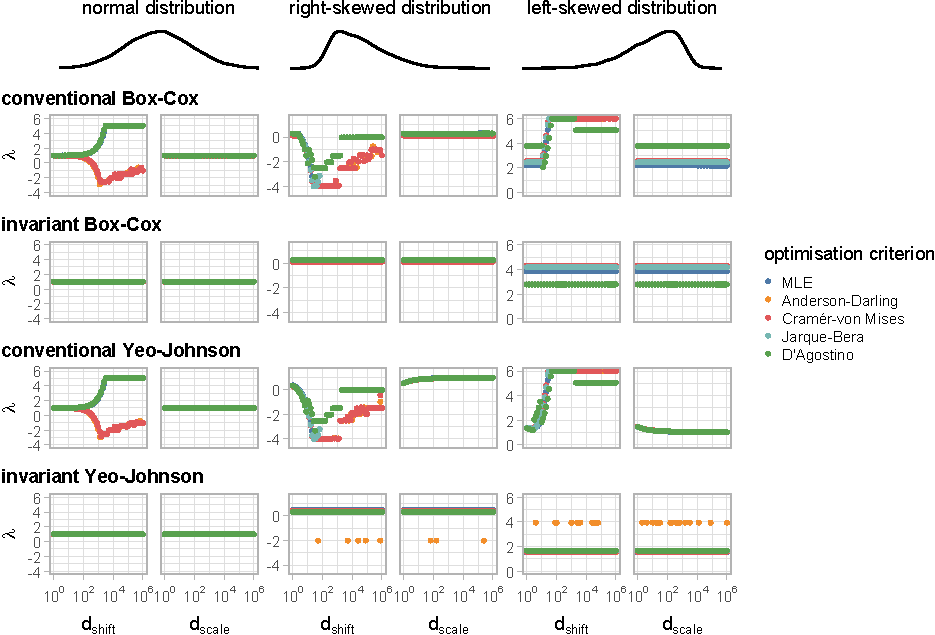
\includegraphics[width=1\linewidth]{appendix_figure_1}

}

\caption{Invariant power transformation produces transformation parameters that are invariant to location and scale. Samples were drawn from normal, right-skewed and left-skewed distributions, respectively, which then underwent a shift $d_{\text{shift}}$ or multiplication by $d_{\text{scale}}$. Estimates of the transformation parameter $\lambda$ for the conventional power transformations show strong dependency on the overall location and scale of the distribution and the optimisation criterion, whereas estimates obtained for the location- and scale-invariant power transformations are constant. For location- and scale-invariant power transformations, the Anderson-Darling criterion leads to unstable estimates of $\lambda$ for skewed distributions, possibly due to large weights being assigned to samples at the upper and lower ends of the distribution.}\label{fig:shifted-distributions-appendix}
\end{figure}

\FloatBarrier



\section{Central normality test and empirical central
normality test critical
values}\label{appendix-c}

Critical values for the central normality test and its empirical variant
are found in Table \ref{tab:central-normality-critical-statistic} and
Table \ref{tab:empirical-central-normality-critical-statistic},
respectively.

\begin{table}
\caption{Critical values of test statistic $\tau_{\alpha, n, \kappa = 0.80}$ for
\textbf{central normality} at $\kappa = 0.80$, as a function of significance 
level $\alpha$ and number of instances $n$. The values shown must be divided by $100$.}
\label{tab:central-normality-critical-statistic}
\begin{tabular}{l | r r r r r r r r r}

\toprule
$n$ \textbackslash $\alpha$ & 0.001 & 0.01 & 0.025 & 0.05 & 0.1 & 0.2 & 0.5 & 0.8 & 0.9 \\

\midrule
    5 & 210.79 & 95.75 & 66.27 & 49.69 & 35.93 & 27.60 & 19.29 & 13.41 & 11.00 \\
   10 &  48.04 & 31.44 & 26.96 & 23.91 & 21.11 & 18.16 & 13.66 & 10.14 &  8.67 \\
   20 &  29.13 & 22.13 & 19.75 & 17.94 & 16.00 & 13.81 & 10.54 &  8.18 &  7.18 \\
   50 &  17.31 & 14.01 & 12.63 & 11.48 & 10.28 &  9.00 &  7.00 &  5.54 &  4.94 \\
  100 &  12.19 & 10.04 &  9.02 &  8.21 &  7.38 &  6.47 &  5.04 &  3.99 &  3.56 \\
  200 &   8.68 &  7.11 &  6.40 &  5.83 &  5.22 &  4.57 &  3.59 &  2.86 &  2.56 \\ 
  500 &   5.61 &  4.54 &  4.08 &  3.70 &  3.33 &  2.91 &  2.28 &  1.82 &  1.63 \\
 1000 &   3.93 &  3.19 &  2.87 &  2.60 &  2.33 &  2.05 &  1.61 &  1.29 &  1.15 \\
 2000 &   2.71 &  2.24 &  2.02 &  1.84 &  1.66 &  1.46 &  1.14 &  0.91 &  0.82 \\
 5000 &   1.73 &  1.42 &  1.28 &  1.17 &  1.05 &  0.92 &  0.72 &  0.58 &  0.52 \\
10000 &   1.22 &  1.00 &  0.90 &  0.82 &  0.74 &  0.65 &  0.51 &  0.41 &  0.37 \\
\bottomrule
\end{tabular}
\end{table}

\begin{table}
\caption{Critical values of test statistic $\tau_{\alpha, n, \kappa = 0.70}$ for
\textbf{empirical central normality} at $\kappa = 0.70$, as a function of significance 
level $\alpha$ and number of instances $n$. The values shown must be divided by $100$.}
\label{tab:empirical-central-normality-critical-statistic}
\begin{tabular}{l | r r r r r r r r r}

\toprule
$n$ \textbackslash $\alpha$ & 0.001 & 0.01 & 0.025 & 0.05 & 0.1 & 0.2 & 0.5 & 0.8 & 0.9 \\

\midrule
    5 & 159.27 & 66.78 & 57.06 & 50.55 & 43.42 & 34.89 & 22.28 & 14.92 & 12.10 \\
   10 &  41.82 & 30.82 & 27.01 & 24.31 & 21.58 & 18.53 & 13.82 & 10.23 &  8.75 \\
   20 &  29.44 & 23.65 & 21.23 & 19.16 & 17.01 & 14.67 & 11.10 &  8.42 &  7.35 \\
   50 &  18.95 & 15.56 & 13.96 & 12.74 & 11.35 &  9.82 &  7.51 &  5.83 &  5.16 \\ 
  100 &  13.49 & 11.00 &  9.91 &  8.98 &  8.03 &  7.04 &  5.43 &  4.25 &  3.76 \\
  200 &   9.65 &  7.99 &  7.22 &  6.64 &  5.96 &  5.21 &  4.05 &  3.17 &  2.81 \\
  500 &   6.37 &  5.32 &  4.82 &  4.44 &  4.03 &  3.57 &  2.79 &  2.18 &  1.92 \\
 1000 &   4.64 &  3.95 &  3.65 &  3.39 &  3.11 &  2.78 &  2.20 &  1.73 &  1.53 \\
 2000 &   3.61 &  3.18 &  2.96 &  2.78 &  2.57 &  2.32 &  1.89 &  1.50 &  1.33 \\
 5000 &   2.78 &  2.48 &  2.36 &  2.24 &  2.11 &  1.95 &  1.66 &  1.39 &  1.25 \\
10000 &   2.39 &  2.18 &  2.08 &  2.00 &  1.91 &  1.81 &  1.59 &  1.39 &  1.28 \\
\bottomrule
\end{tabular}
\end{table}

\begin{figure}

{\centering 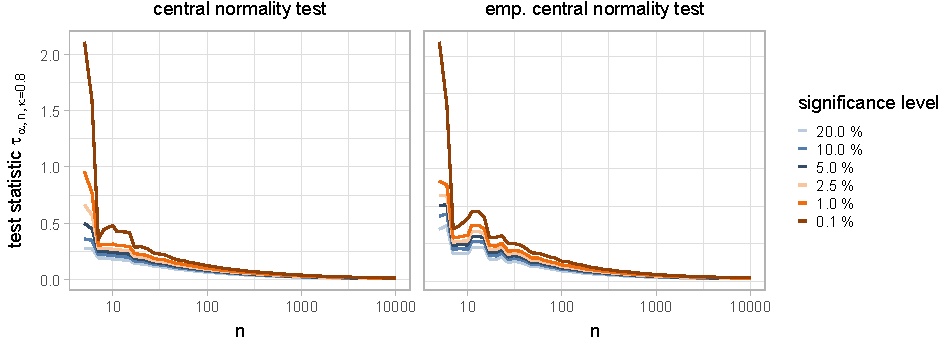
\includegraphics[width=1\linewidth]{appendix_figure_2}

}

\caption{Critical test statistic $\tau_{\alpha, n, \kappa = 0.80}$ of the (empirical) central normality test as function of $n$ for several values of significance level $\alpha$. The critical test statistics for central normality test are determined using fully normal data, whereas the statistics for the empirical variant are determined using centrally normal data, i.e. with fully normal data where 10\% of elements are replaced by outliers. emp: empirical}\label{fig:empirical-central-normality-critical-statistics}
\end{figure}

\FloatBarrier



\section{Assessing transformations using simulated
data}\label{appendix-d}

\subsection{Ranking Box-Cox
transformations}\label{ranking-box-cox-transformations}

Box-Cox transformations were assessed in the same manner as Yeo-Johnson
transformations. The results are shown in Table
\ref{tab:comparison_methods_simulations_box_cox}.

\begin{table}
\caption{
Comparison of average rank between Box-Cox transformation methods based on either residual error (without outliers) or residual error of the central portion
(with outliers; $\kappa = 0.80$) over 3 datasets with 10000 sequences each. The clean dataset consists of sequences derived through inverse Box-Cox transformation
of data sampled from a standard normal distribution. The dirty dataset contains sequences sampled from asymmetric generalised normal distributions.
The shifted dataset also contains sequences sampled from asymmetric generalised normal distributions, but centred at 100, and scaled by 0.001.
If necessary, each sequence was shifted so that every element had a strictly positive value. 
Several transformation methods include normalisation before transformation, indicated by z-score normalisation (norm.) or robust scaling.
A rank of 1 is the best and a rank of 9 the worst. For each dataset, the best ranking transformation is marked in bold.
}
\label{tab:comparison_methods_simulations_box_cox}
\begin{tabular}{l | l r r r r r r}

\toprule
& dataset: & \multicolumn{2}{c}{clean} & \multicolumn{2}{c}{dirty} & \multicolumn{2}{c}{shifted} \\
transformation & outliers: & no & yes & no & yes & no & yes \\

\midrule

none                                  & &         7.65  &         6.96  &         7.28  &         6.58  &         7.45  &         6.78 \\
conventional                          & &         3.10  &         5.98  &         5.42  &         6.16  &         6.49  &         6.10 \\
conventional (z-score norm.)          & &         4.19  &         6.28  &         4.85  &         6.33  &         4.38  &         5.85 \\
conventional (robust scaling)         & &         4.20  &         6.28  &         4.78  &         6.33  &         4.30  &         5.86 \\
Raymaekers-Rousseeuw                  & &         4.46  &         3.55  &         5.39  &         3.69  &         6.29  &         5.84 \\ 
Raymaekers-Rousseeuw (z-score norm.)  & &         6.21  &         3.83  &         4.95  &         3.85  &         4.51  &         3.50 \\ 
Raymaekers-Rousseeuw (robust scaling) & &         6.12  &         3.82  &         4.97  &         3.85  &         4.52  &         3.50 \\
invariant                             & & \textbf{2.99} &         5.55  & \textbf{3.65} &         6.01  & \textbf{3.52} &         5.57 \\
robust invariant                      & &         6.09  & \textbf{2.75} &         3.71  & \textbf{2.20} &         3.55  & \textbf{2.00} \\

\bottomrule
\end{tabular}
\end{table}

\FloatBarrier




\subsection{Examples using clean data}\label{examples-using-clean-data}

Robust transformations are hypothesised to have a cost in efficiency for
data without outliers, i.e.~clean data. Here we draw nine sequences with
elements randomly drawn from a standard normal distribution
\(\mathcal{N}(0,1)\). Subsequently, we perform an inverse transformation
\(\left(\phi^{\lambda, 0, 1}\right)^{-1}\), with
\(\lambda \in \left(0, 2\right)\).

The sequences drawn resulted from the permutations of the number of
elements of each sequence (\(n \in \{30, 100, 500\}\)) and
transformation parameter for the inverse transformation
\(\lambda \in \{0.1, 1.0, 1.9\}\). Each sequence then underwent power
transformation using Box-Cox and Yeo-Johnson transformations. For
Box-Cox transformations, each sequence was shifted prior to inverse
transformation so that every element after inverse transformation would
be strictly positive.

Results for Box-Cox transformations are shown in Table
\ref{tab:clean-transformation-appendix-residuals-bc},
\ref{tab:clean-transformation-appendix-lambda-bc}, and
\ref{tab:clean-transformation-appendix-p-value-bc}. Additionally,
results for Yeo-Johnson transformations are shown in Table
\ref{tab:clean-transformation-appendix-residuals-yj},
\ref{tab:clean-transformation-appendix-lambda-yj}, and
\ref{tab:clean-transformation-appendix-p-value-yj}. As may be observed,
in these examples robust location- and shift-invariant transformations
have higher residual errors because of low weights being assigned to
tails of a distribution. This is also shown in Tables
\ref{tab:comparison_methods_simulations_yeo_johnson} and
\ref{tab:comparison_methods_simulations_box_cox} for clean data without
outliers.

\begin{table}
\caption{Residual errors for features from simulated clean data without outliers after Yeo-Johnson transformation to normality.
Several transformation methods include normalisation before transformation, indicated by z-score normalisation (norm.) or robust scaling.}
\label{tab:clean-transformation-appendix-residuals-yj}
\small{
\begin{tabular}{l | l r r r r r r r r r}

\toprule
& n: & \multicolumn{3}{c}{30} & \multicolumn{3}{c}{100} & \multicolumn{3}{c}{500} \\
transformation & $\lambda$: & 0.1 & 1.0 & 1.9 & 0.1 & 1.0 & 1.9 & 0.1 & 1.0 & 1.9 \\

\midrule

none                                  & & 4.0 & 3.4 & 4.6 & 40.1 &  8.9 & 20.8 & 184.6 & 10.1 & 191.8 \\
conventional                          & & 2.7 & 3.3 & 3.6 &  6.5 &  8.1 &  5.6 &  14.2 & 10.1 &  16.1 \\
conventional (z-score norm.)          & & 2.5 & 3.3 & 3.7 &  9.8 &  8.1 &  5.6 &  24.1 & 10.1 &  15.9 \\
conventional (robust scaling)         & & 2.6 & 3.3 & 3.7 &  7.4 &  8.2 &  5.6 &  15.5 & 10.1 &  14.0 \\
Raymaekers-Rousseeuw                  & & 3.8 & 3.3 & 3.6 &  6.5 &  8.5 &  5.6 &  14.4 & 11.0 &  17.6 \\
Raymaekers-Rousseeuw (z-score norm.)  & & 2.6 & 3.3 & 3.7 &  9.8 &  8.5 &  5.6 &  24.1 & 11.1 &  15.9 \\
Raymaekers-Rousseeuw (robust scaling) & & 2.6 & 3.3 & 3.7 &  7.4 &  8.6 &  5.6 &  15.4 & 11.1 &  15.1 \\
invariant                             & & 3.0 & 3.5 & 3.6 &  5.0 &  8.1 &  5.6 &  13.1 & 10.9 &  17.8 \\
robust invariant                      & & 3.0 & 3.4 & 3.6 &  5.5 & 10.1 &  6.2 &  18.7 & 13.2 &  32.8 \\

\bottomrule
\end{tabular}
}
\end{table}

\begin{table}
\caption{Transformation parameter $\lambda$ for features from simulated clean data without outliers after Yeo-Johnson transformation to normality.
Several transformation methods include normalisation before transformation, indicated by z-score normalisation (norm.) or robust scaling.}
\label{tab:clean-transformation-appendix-lambda-yj}
\small{
\begin{tabular}{l | l r r r r r r r r r}

\toprule
& n: & \multicolumn{3}{c}{30} & \multicolumn{3}{c}{100} & \multicolumn{3}{c}{500} \\
transformation & $\lambda$: & 0.1 & 1.0 & 1.9 & 0.1 & 1.0 & 1.9 & 0.1 & 1.0 & 1.9 \\

\midrule

conventional                          & & 0.6 & 1.2 & 1.5 &  0.0 & 0.9 & 1.6 &  0.1 & 1.0 & 1.9 \\
conventional (z-score norm.)          & & 0.5 & 1.2 & 1.5 & -0.2 & 0.9 & 1.7 & -0.2 & 1.0 & 2.2 \\
conventional (robust scaling)         & & 0.5 & 1.3 & 1.6 & -0.3 & 0.9 & 1.7 & -0.2 & 1.0 & 2.1 \\
Raymaekers-Rousseeuw                  & & 1.0 & 1.2 & 1.5 &  0.0 & 0.7 & 1.6 &  0.1 & 1.0 & 1.9 \\
Raymaekers-Rousseeuw (z-score norm.)  & & 0.7 & 1.2 & 1.5 & -0.2 & 0.7 & 1.7 & -0.2 & 1.0 & 2.2 \\
Raymaekers-Rousseeuw (robust scaling) & & 0.6 & 1.3 & 1.6 & -0.3 & 0.6 & 1.7 & -0.2 & 1.0 & 2.1 \\
invariant                             & & 0.4 & 1.4 & 1.7 &  0.1 & 0.9 & 1.8 &  0.1 & 1.1 & 3.0 \\
robust invariant                      & & 0.5 & 1.1 & 1.5 & -0.1 & 0.7 & 1.7 &  0.1 & 1.1 & 1.9 \\
\bottomrule
\end{tabular}
}
\end{table}

\begin{table}
\caption{
p-values of empirical central normality tests for features from simulated clean data without outliers after Yeo-Johnson transformation to normality.
Several transformation methods include normalisation before transformation, indicated by z-score normalisation (norm.) or robust scaling.}
\label{tab:clean-transformation-appendix-p-value-yj}
\small{
\begin{tabular}{p{3.5cm} | l r r r r r r r r r}

\toprule
& n: & \multicolumn{3}{c}{30} & \multicolumn{3}{c}{100} & \multicolumn{3}{c}{500} \\
transformation & $\lambda$: & 0.1 & 1.0 & 1.9 & 0.1 & 1.0 & 1.9 & 0.1 & 1.0 & 1.9 \\

\midrule

none                                  & & 0.981 & 0.816 & 0.576 & $<0.001$ & 0.099 & 0.011 & $<0.001$ & 0.993 & $<0.001$ \\
conventional                          & & 0.979 & 0.614 & 0.617 &   0.722  & 0.221 & 0.782 &   0.946  & 0.997 &   0.637 \\
conventional (z-score norm.)          & & 0.970 & 0.594 & 0.645 &   0.251  & 0.224 & 0.895 &   0.529  & 0.998 &   0.828 \\
conventional (robust scaling)         & & 0.974 & 0.593 & 0.640 &   0.538  & 0.207 & 0.837 &   0.933  & 0.998 &   0.810 \\
Raymaekers-Rousseeuw                  & & 0.983 & 0.614 & 0.617 &   0.722  & 0.622 & 0.782 &   0.927  & 0.985 &   0.831 \\
Raymaekers-Rousseeuw (z-score norm.)  & & 0.985 & 0.594 & 0.645 &   0.251  & 0.623 & 0.895 &   0.564  & 0.984 &   0.807 \\
Raymaekers-Rousseeuw (robust scaling) & & 0.987 & 0.593 & 0.640 &   0.538  & 0.599 & 0.837 &   0.935  & 0.984 &   0.875 \\
invariant                             & & 0.987 & 0.487 & 0.573 &   0.778  & 0.241 & 0.683 &   0.963  & 0.997 &   0.865 \\
robust invariant                      & & 0.992 & 0.753 & 0.667 &   0.909  & 0.739 & 0.628 &   0.968  & 0.994 &   0.680 \\

\bottomrule
\end{tabular}
}
\end{table}

\begin{table}
\caption{Residual errors for features from simulated clean data without outliers after Box-Cox transformation to normality.
Several transformation methods include normalisation before transformation, indicated by z-score normalisation (norm.) or robust scaling.}
\label{tab:clean-transformation-appendix-residuals-bc}
\small{
\begin{tabular}{l | l r r r r r r r r r}

\toprule
& n: & \multicolumn{3}{c}{30} & \multicolumn{3}{c}{100} & \multicolumn{3}{c}{500} \\
transformation & $\lambda$: & 0.1 & 1.0 & 1.9 & 0.1 & 1.0 & 1.9 & 0.1 & 1.0 & 1.9 \\

\midrule

none                                  & & 5.3 & 3.4 & 3.8 & 45.7 &  8.9 & 6.0 & 221.8 & 10.1 & 29.7 \\
conventional                          & & 2.4 & 3.2 & 3.5 &  5.9 &  8.4 & 5.5 &  14.3 &  9.8 & 16.1 \\
conventional (z-score norm.)          & & 2.4 & 3.2 & 3.7 &  5.4 &  8.7 & 5.5 &  14.0 & 10.4 & 16.1 \\
conventional (robust scaling)         & & 2.4 & 3.2 & 3.7 &  5.4 &  8.7 & 5.5 &  14.0 & 10.4 & 16.1 \\
Raymaekers-Rousseeuw                  & & 2.4 & 3.2 & 3.5 &  5.9 & 13.3 & 5.7 &  16.1 & 13.6 & 16.9 \\
Raymaekers-Rousseeuw (z-score norm.)  & & 2.4 & 3.2 & 4.9 &  6.3 &  8.9 & 6.2 &  19.1 & 19.0 & 19.9 \\
Raymaekers-Rousseeuw (robust scaling) & & 2.4 & 3.2 & 4.9 &  6.3 &  8.9 & 6.2 &  18.4 & 19.0 & 19.9 \\
invariant                             & & 2.4 & 3.2 & 3.7 &  5.4 &  8.7 & 5.5 &  13.7 &  9.9 & 16.0 \\
robust invariant                      & & 2.4 & 4.3 & 4.7 &  8.9 & 20.4 & 6.7 &  14.1 & 15.8 & 37.6 \\

\bottomrule
\end{tabular}
}
\end{table}

\begin{table}
\caption{Transformation parameter $\lambda$ for features from simulated clean data without outliers after Box-Cox transformation to normality.
Several transformation methods include normalisation before transformation, indicated by z-score normalisation (norm.) or robust scaling.}
\label{tab:clean-transformation-appendix-lambda-bc}
\small{
\begin{tabular}{l | l r r r r r r r r r}

\toprule
& n: & \multicolumn{3}{c}{30} & \multicolumn{3}{c}{100} & \multicolumn{3}{c}{500} \\
transformation & $\lambda$: & 0.1 & 1.0 & 1.9 & 0.1 & 1.0 & 1.9 & 0.1 & 1.0 & 1.9 \\

\midrule

conventional                          & & 0.4 & 1.3 & 0.5 & 0.0 &  0.9 & 0.7 & 0.1 & 1.1 & 2.0 \\
conventional (z-score norm.)          & & 0.4 & 1.1 & 0.8 & 0.2 &  0.9 & 0.8 & 0.1 & 1.0 & 1.4 \\
conventional (robust scaling)         & & 0.4 & 1.1 & 0.8 & 0.2 &  0.9 & 0.8 & 0.1 & 1.0 & 1.4 \\
Raymaekers-Rousseeuw                  & & 0.4 & 1.3 & 0.5 & 0.0 & -0.1 & 0.5 & 0.1 & 0.9 & 1.8 \\
Raymaekers-Rousseeuw (z-score norm.)  & & 0.4 & 1.1 & 0.4 & 0.1 &  0.8 & 0.7 & 0.1 & 0.9 & 1.2 \\
Raymaekers-Rousseeuw (robust scaling) & & 0.4 & 1.1 & 0.4 & 0.1 &  0.8 & 0.7 & 0.1 & 0.9 & 1.2 \\
invariant                             & & 0.4 & 1.6 & 0.8 & 0.2 &  0.9 & 0.8 & 0.1 & 1.1 & 1.9 \\
robust invariant                      & & 0.5 & 0.8 & 0.4 & 0.0 &  0.2 & 0.7 & 0.1 & 0.9 & 0.9 \\

\bottomrule
\end{tabular}
}
\end{table}

\begin{table}
\caption{
p-values of empirical central normality tests for features from simulated clean data without outliers after Box-Cox transformation to normality.
Several transformation methods include normalisation before transformation, indicated by z-score normalisation (norm.) or robust scaling.}
\label{tab:clean-transformation-appendix-p-value-bc}
\small{
\begin{tabular}{p{3.5cm} | l r r r r r r r r r}

\toprule
& n: & \multicolumn{3}{c}{30} & \multicolumn{3}{c}{100} & \multicolumn{3}{c}{500} \\
transformation & $\lambda$: & 0.1 & 1.0 & 1.9 & 0.1 & 1.0 & 1.9 & 0.1 & 1.0 & 1.9 \\

\midrule

none                                  & & 0.940 & 0.816 & 0.498 & $<0.001$ & 0.098 & 0.714 & $<0.001$ & 0.993 & 0.928 \\
conventional                          & & 0.948 & 0.695 & 0.603 &   0.798  & 0.163 & 0.791 &   0.931  & 0.997 & 0.658 \\
conventional (z-score norm.)          & & 0.947 & 0.777 & 0.624 &   0.611  & 0.182 & 0.788 &   0.969  & 0.991 & 0.822 \\
conventional (robust scaling)         & & 0.947 & 0.777 & 0.624 &   0.611  & 0.182 & 0.788 &   0.969  & 0.991 & 0.822 \\
Raymaekers-Rousseeuw                  & & 0.948 & 0.695 & 0.603 &   0.798  & 0.768 & 0.806 &   0.816  & 0.962 & 0.782 \\
Raymaekers-Rousseeuw (z-score norm.)  & & 0.947 & 0.777 & 0.753 &   0.913  & 0.255 & 0.784 &   0.775  & 0.866 & 0.921 \\
Raymaekers-Rousseeuw (robust scaling) & & 0.947 & 0.777 & 0.753 &   0.913  & 0.255 & 0.784 &   0.807  & 0.866 & 0.921 \\
invariant                             & & 0.947 & 0.661 & 0.624 &   0.611  & 0.182 & 0.789 &   0.956  & 0.997 & 0.664 \\
robust invariant                      & & 0.969 & 0.824 & 0.750 &   0.972  & 0.779 & 0.775 &   0.956  & 0.934 & 0.840 \\

\bottomrule
\end{tabular}
}
\end{table}

\FloatBarrier




\section{Experimental
results}\label{appendix-e}

The effect of using location- and scale-invariant transformations was
investigated using real-world datasets, as described in the main
manuscript.

\subsection{Yeo-Johnson
transformation}\label{yeo-johnson-transformation}

Additional results for Yeo-Johnson transformations are shown in Tables
\ref{tab:experimental-results-appendix-residuals},
\ref{tab:experimental-results-appendix-lambda},
\ref{tab:experimental-results-appendix-p-value}.

\begin{table}
\caption{Residual errors for features from real-world datasets after Yeo-Johnson transformation to normality. 
Several transformation methods include normalisation before transformation, indicated by z-score normalisation (norm.) or robust scaling. 
AWT: arterial wall thickness; FE: fuel efficiency; PBM: penguin body mass}
\label{tab:experimental-results-appendix-residuals}
\begin{tabular}{l | r r r r r}

\toprule
feature & age & AWT & FE & latitude & PBM \\

\midrule
none                                  & 16.5 & 110.1 & 54.5 & 328.4 & 48.0 \\
conventional                          & 11.5 &  30.0 & 55.3 & 319.0 & 32.2 \\
conventional (z-score norm.)          & 11.5 &  19.3 & 49.0 & 326.2 & 33.3 \\
conventional (robust scaling)         & 11.3 &  31.8 & 53.3 & 324.5 & 32.2 \\
Raymaekers-Rousseeuw                  & 11.5 & 136.7 & 47.7 & 315.1 & 32.2 \\
Raymaekers-Rousseeuw (z-score norm.)  & 13.2 & 214.5 & 57.4 & 326.2 & 33.3 \\
Raymaekers-Rousseeuw (robust scaling) & 11.7 & 281.3 & 57.0 & 324.5 & 32.0 \\
invariant                             &  8.8 &  12.2 & 44.0 & 326.4 & 26.8 \\
robust invariant                      &  9.3 &  30.2 & 55.8 & 308.1 & 22.0 \\

\bottomrule
\end{tabular}
\end{table}

\begin{table}
\caption{Transformation parameter $\lambda$ for features from real-world datasets after Yeo-Johnson transformation to normality. 
Several transformation methods include normalisation before transformation, indicated by z-score normalisation (norm.) or robust scaling. 
AWT: arterial wall thickness; FE: fuel efficiency; PBM: penguin body mass}
\label{tab:experimental-results-appendix-lambda}
\begin{tabular}{l | r r r r r}

\toprule
feature & age & AWT & FE & latitude & PBM \\

\midrule
conventional                          & 2.0 & -0.7 & -0.1 & 62.1 & -0.5 \\
conventional (z-score norm.)          & 1.2 & -1.7 & -0.1 &  1.3 &  0.6 \\
conventional (robust scaling)         & 1.3 &  0.0 &  0.2 &  1.4 &  0.4 \\
Raymaekers-Rousseeuw                  & 2.0 &  1.1 &  0.8 & 95.4 & -0.5 \\
Raymaekers-Rousseeuw (z-score norm.)  & 1.3 &  1.4 &  1.0 &  1.3 &  0.6 \\
Raymaekers-Rousseeuw (robust scaling) & 1.4 &  1.3 &  1.0 &  1.4 &  0.4 \\
invariant                             & 1.3 &  0.2 & -1.3 &  1.5 &  0.5 \\
robust invariant                      & 1.3 & -0.3 &  1.0 &  1.1 &  0.3 \\
\bottomrule
\end{tabular}
\end{table}

\begin{table}
\caption{
p-values of empirical central normality tests for features from real-world datasets after Yeo-Johnson transformation to normality.
Several transformation methods include normalisation before transformation, indicated by z-score normalisation (norm.) or robust scaling. 
AWT: arterial wall thickness; FE: fuel efficiency; PBM: penguin body mass}
\label{tab:experimental-results-appendix-p-value}
\begin{tabular}{l | r r r r r}

\toprule
feature & age & AWT & FE & latitude & PBM \\

\midrule

none                                  & 0.694 & 0.832     & 0.727     & $< 0.001$ & $< 0.001$ \\
conventional                          & 0.961 & 0.003     & $< 0.001$ & $< 0.001$ & 0.101 \\
conventional (z-score norm.)          & 0.919 & 0.021     & $< 0.001$ & $< 0.001$ & 0.099 \\
conventional (robust scaling)         & 0.933 & $< 0.001$ & $< 0.001$ & $< 0.001$ & 0.129 \\
Raymaekers-Rousseeuw                  & 0.961 & 0.881     & 0.373     & $< 0.001$ & 0.101 \\
Raymaekers-Rousseeuw (z-score norm.)  & 0.694 & 0.899     & 0.809     & $< 0.001$ & 0.099 \\
Raymaekers-Rousseeuw (robust scaling) & 0.900 & 0.880     & 0.811     & $< 0.001$ & 0.144 \\
invariant                             & 0.976 & 0.147     & $< 0.001$ & $< 0.001$ & 0.276 \\
robust invariant                      & 0.933 & 0.178     & 0.759     & $< 0.001$ & 0.688 \\

\bottomrule
\end{tabular}
\end{table}

\FloatBarrier

\subsection{Box-Cox transformation}\label{box-cox-transformation}

Results for Box-Cox transformations are shown in Tables
\ref{tab:experimental-results-appendix-residuals-bc},
\ref{tab:experimental-results-appendix-lambda-bc} and
\ref{tab:experimental-results-appendix-p-value-bc}.

\begin{table}
\caption{Residual errors for features from real-world datasets after Box-Cox transformation to normality. 
Several transformation methods include normalisation before transformation, indicated by z-score normalisation (norm.) or robust scaling. 
AWT: arterial wall thickness; FE: fuel efficiency; PBM: penguin body mass}
\label{tab:experimental-results-appendix-residuals-bc}
\begin{tabular}{l | r r r r r}

\toprule
feature & age & AWT & FE & latitude & PBM \\

\midrule
none                                  & 16.5 & 110.1 &  54.5 & 328.4 & 48.0 \\
conventional                          & 11.5 &  33.5 &  55.7 & 318.9 & 32.2 \\
conventional (z-score norm.)          & 12.9 &  44.5 &  58.8 & 305.3 & 27.3 \\
conventional (robust scaling)         & 12.9 &  44.7 &  59.0 & 305.3 & 27.3 \\
Raymaekers-Rousseeuw                  & 11.5 & 127.1 &  47.6 & 314.8 & 32.2 \\ 
Raymaekers-Rousseeuw (z-score norm.)  & 13.1 &  54.8 & 127.5 & 510.2 & 23.6 \\
Raymaekers-Rousseeuw (robust scaling) & 18.9 & 100.2 & 113.7 & 510.2 & 23.6 \\
invariant                             & 11.6 &  28.0 &  48.4 & 311.8 & 27.3 \\
robust invariant                      & 12.8 & 150.1 &  60.5 & 646.0 & 27.4 \\

\bottomrule
\end{tabular}
\end{table}

\begin{table}
\caption{Transformation parameter $\lambda$ for features from real-world datasets after Box-Cox transformation to normality. 
Several transformation methods include normalisation before transformation, indicated by z-score normalisation (norm.) or robust scaling. 
AWT: arterial wall thickness; FE: fuel efficiency; PBM: penguin body mass}
\label{tab:experimental-results-appendix-lambda-bc}
\begin{tabular}{l | r r r r r}

\toprule
feature & age & AWT & FE & latitude & PBM \\

\midrule

conventional                          & 1.9 & -0.5 & -0.1 & 62.1 & -0.5 \\
conventional (z-score norm.)          & 1.2 &  0.1 &  0.2 &  1.2 &  0.5 \\
conventional (robust scaling)         & 1.2 &  0.1 &  0.1 &  1.2 &  0.5 \\
Raymaekers-Rousseeuw                  & 1.9 &  1.1 &  0.8 & 95.9 & -0.5 \\
Raymaekers-Rousseeuw (z-score norm.)  & 1.2 &  0.6 & -0.5 &  0.6 &  0.3 \\
Raymaekers-Rousseeuw (robust scaling) & 0.9 &  1.0 & -0.5 &  0.6 &  0.3 \\
invariant                             & 1.7 & -1.0 & -0.7 &  1.9 &  0.5 \\
robust invariant                      & 1.3 &  1.2 &  1.1 &  0.4 &  0.1 \\

\bottomrule
\end{tabular}
\end{table}

\begin{table}
\caption{
p-values of empirical central normality tests for features from real-world datasets after Box-Cox transformation to normality.
Several transformation methods include normalisation before transformation, indicated by z-score normalisation (norm.) or robust scaling. 
AWT: arterial wall thickness; FE: fuel efficiency; PBM: penguin body mass}
\label{tab:experimental-results-appendix-p-value-bc}
\begin{tabular}{l | r r r r r}

\toprule
feature & age & AWT & FE & latitude & PBM \\

\midrule

none                                  & 0.694 & 0.832 & 0.727     & $< 0.001$ & $< 0.001$ \\
conventional                          & 0.961 & 0.002 & $< 0.001$ & $< 0.001$ & 0.101 \\
conventional (z-score norm.)          & 0.901 & 0.005 & $< 0.001$ & $< 0.001$ & 0.154 \\
conventional (robust scaling)         & 0.901 & 0.005 & $< 0.001$ & $< 0.001$ & 0.154 \\
Raymaekers-Rousseeuw                  & 0.961 & 0.871 & 0.365     & $< 0.001$ & 0.101 \\
Raymaekers-Rousseeuw (z-score norm.)  & 0.891 & 0.268 & $< 0.001$ & $< 0.001$ & 0.495 \\
Raymaekers-Rousseeuw (robust scaling) & 0.562 & 0.789 & $< 0.001$ & $< 0.001$ & 0.492 \\
invariant                             & 0.962 & 0.004 & $< 0.001$ & $< 0.001$ & 0.154 \\
robust invariant                      & 0.899 & 0.890 & 0.866     & $< 0.001$ & 0.622 \\

\bottomrule
\end{tabular}
\end{table}

\FloatBarrier

\end{appendices}

%%===========================================================================================%%
%% If you are submitting to one of the Nature Portfolio journals, using the eJP submission   %%
%% system, please include the references within the manuscript file itself. You may do this  %%
%% by copying the reference list from your .bbl file, paste it into the main manuscript .tex %%
%% file, and delete the associated \verb+\bibliography+ commands.                            %%
%%===========================================================================================%%

\bibliography{refs}% common bib file
%% if required, the content of .bbl file can be included here once bbl is generated
%%\input sn-article.bbl


\end{document}
